%\pdfoutput=1
% \documentclass[12pt,a4paper,superscriptaddress,preprint,longbibliography]{revtex4-1}
\documentclass[20pt]{extarticle}
% http://www-math.mit.edu/~psh/amshelp/2.3/template.tex
\usepackage[dvips]{graphicx}

\usepackage{mathtools}

\usepackage{geometry}
	\geometry{
	left=3mm,
	right=3mm,
	top=3mm,
	bottom=9mm,
	includefoot,
	footskip=5mm
	}

\usepackage{amssymb,amsmath}

\renewcommand{\labelitemii}{$\blacktriangleright$}

\usepackage{bm}
\usepackage{color}

\usepackage{esvect}

\usepackage{supertabular}
\usepackage{multirow}
\usepackage{bigstrut}

\usepackage{ulem}
\newcommand{\del}[1]{\textcolor{red}{\sout{#1}}}
\newcommand{\ms}[1]{\textcolor{orange}{\bf [Michiko: #1]}}
\newcommand{\add}[1]{\textcolor{blue}{#1}}
\newcommand{\addd}[1]{\textcolor{orange}{#1}}
\newcommand{\naoki}[1]{\textcolor{green}{\bf [Naoki: #1]}}
\newcommand{\tw}[1]{\textcolor{cyan}{\bf [Takamitsu: #1]}}

\usepackage[hidelinks]{hyperref}
\newcommand{\hrefc}[2]{\href{#1}{\textcolor{blue}{#2}}}

\newcommand{\topdir}{../../..}

% Page number: bottom right, small font, on every page (incl. title page).
\usepackage{fancyhdr}
\pagestyle{fancy}
\fancyhf{}
\renewcommand{\headrulewidth}{0pt}
\renewcommand{\footrulewidth}{0pt}
\fancyfoot[R]{\footnotesize\thepage}
\fancypagestyle{plain}{%
	\fancyhf{}%
	\renewcommand{\headrulewidth}{0pt}%
	\renewcommand{\footrulewidth}{0pt}%
	\fancyfoot[R]{\footnotesize\thepage}%
}

\sloppy

\begin{document}

\title{MATH 463 Mathematical Biology\\ lecture notes\\
9. Network biology and network medicine}
\date{\today}
\author{Naoki Masuda}

\maketitle

\begin{itemize}
\item \hrefc{https://network-science-notes.github.io/}{A useful lecture note on network science.}
\item A full exposure to network science:
	\begin{itemize}
	\item CMPLXSYS 335: Introduction to Network Science
	\end{itemize}
\end{itemize}

\subsection*{Network and adjacency matrix}

\subsubsection*{Network and graph}

\begin{itemize}
\item A graph $G = (V, E)$, where
	\begin{itemize}
	\item $V = (v_1, v_2, \ldots, v_N)$ is the set of nodes (also called vertices),
	\item $N$ is the number of nodes, and
	\item $E$ is the set of edges (also called links, arcs, ties). An edge, $(v_i, v_j)$, represents a pairwise relation between \emph{two} nodes.
	\end{itemize}
\item Graph and network mean the same thing.
	\begin{itemize}
	\item Graph theory and network science. What is the difference between the two?
	\end{itemize}
\item A network may be directed (edges are ordered pairs of nodes) or undirected (edges are unordered pairs of nodes). Examples?
\item A network may be weighted (edges with weight) or unweighted (an edge is only either present or absent between each node pair).
\end{itemize}

\subsubsection*{Adjacency matrix}

\begin{itemize}
\item $N\times N$ adjacency matrix $A = (A_{ij})$, where
\[
A_{ij} = \begin{cases}
1 & \text{if } (i, j) \in E,\\
0 & \text{otherwise}.
\end{cases}
\]
\end{itemize}

\noindent\textbf{Exercise:} Write the adjacency matrix of this network:

\begin{flushleft}
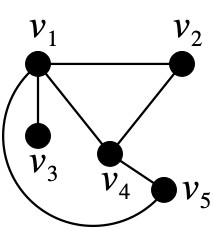
\includegraphics[width=0.3\textwidth]{figures/9_networks/net-example-kk.png}
\end{flushleft}

\begin{itemize}
\item This is already \emph{mathematical modeling} of networks.
	\begin{itemize}
	\item Network modeling is not a dynamics modeling.
		\begin{itemize}
		\item We have been studying dynamics modeling in almost all weeks.
		\item But I insist that math biology does not imply dynamics.
		\end{itemize}
	\end{itemize}
\item \textbf{Question:} In general, which is more difficult to theoretically analyze, directed unweighted networks or undirected weighted networks?
\end{itemize}

\subsection*{Measurements and facts about empirical networks}

\begin{center}
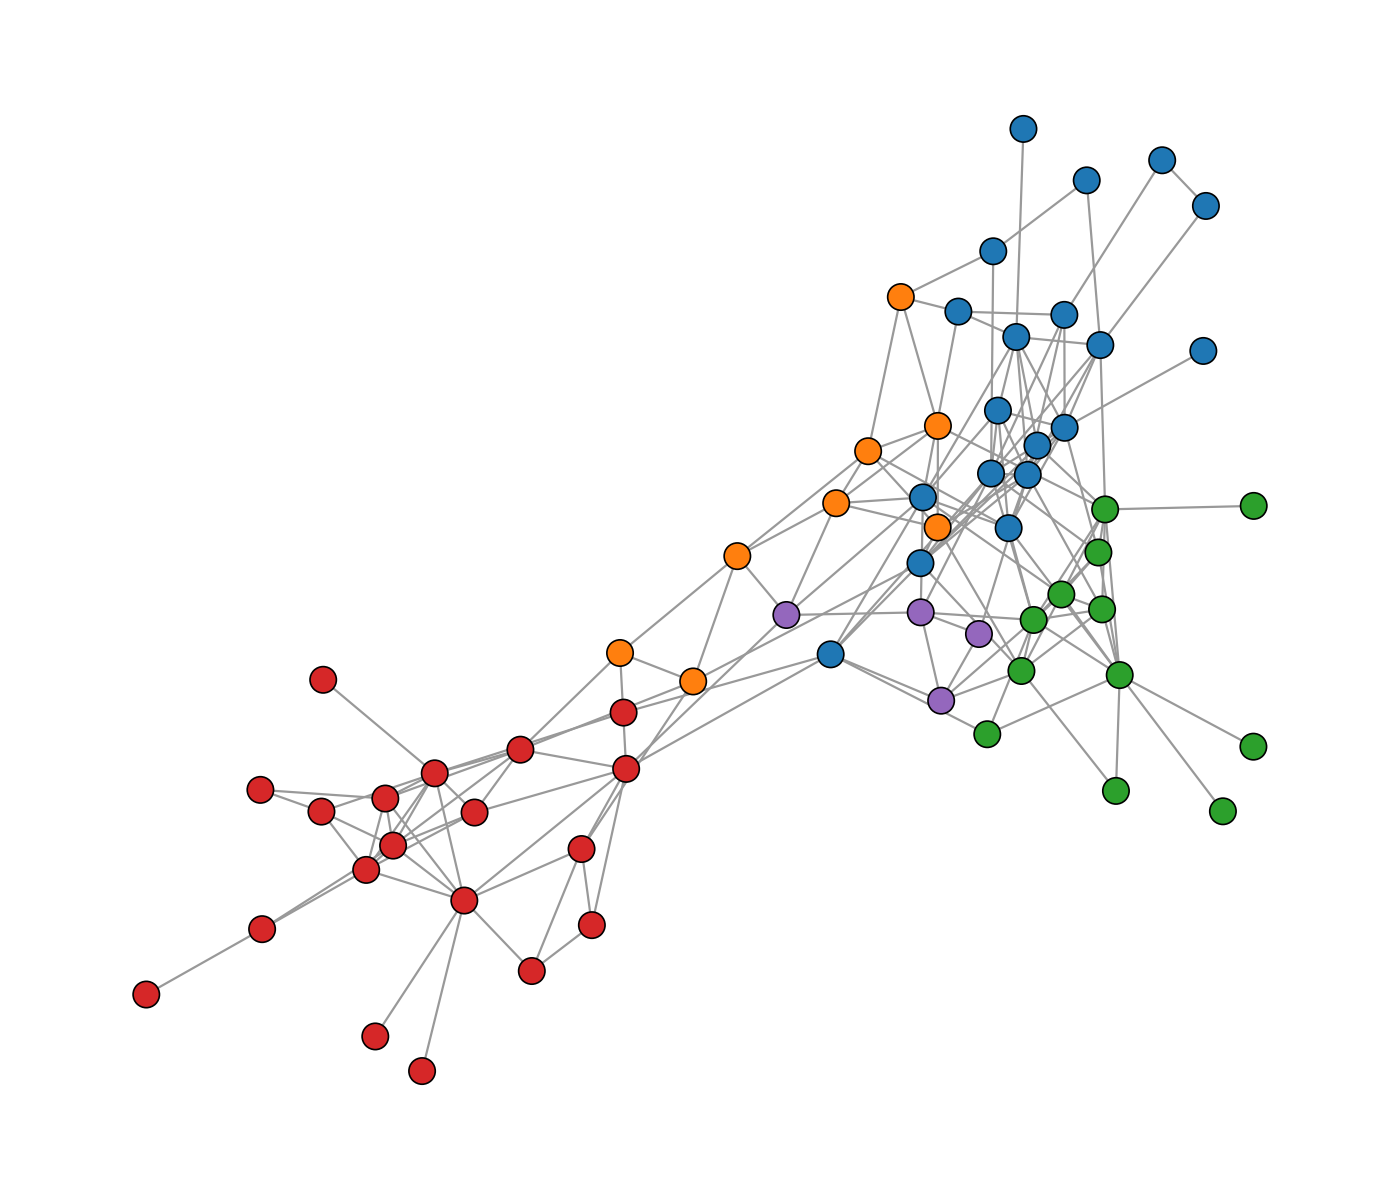
\includegraphics[width=0.6\textwidth]{figures/9_networks/dolphins-network.png}
\end{center}
Figure: A social network of 62 bottlenose dolphins living off Doubtful Sound, New Zealand. An edge means that two dolphins were frequently seen together. The colors show communities found by an algorithm (modularity maximization). Drawn from the data of \hrefc{https://doi.org/10.1007/s00265-003-0651-y}{Lusseau et al., Behav.\ Ecol.\ Sociobiol.\ (2003)}; the community structure of this network was analyzed in \hrefc{https://doi.org/10.1098/rsbl.2004.0225}{Lusseau and Newman, Proc R Soc B (2004)}.


\begin{enumerate}
\item Degree (of a node), $k$ (sometimes $d$): the number of neighbors that a node has.
	\begin{itemize}
	\item Degree distribution, $p(k)$: fraction of nodes in a network that have degree $k$.
		\begin{itemize}
		\item In the above network, $p(k) = \frac{1}{5}\delta_{k,1} + \frac{2}{5} \delta_{k, 2} + \frac{1}{5} \delta_{k,3} + \frac{1}{5} \delta_{k, 4}$.
		\end{itemize}
	\item The degree distribution is often power-law-like (called scale-free, heavy-tailed, fat-tailed, long-tailed).
	\item $p(k) = C k^{-\gamma}$, where often $2<\gamma<3$.
	\item $\bar{F}(k) = \int_k^{\infty} p(k') \text{d}k'$, called the survival function or complementary cumulative function.
	\item \textbf{Q:} Compute $\bar{F}(k)$ for $p(k) = C k^{-\gamma}$.
	\item \textbf{Q:} Take log of $p(k) = C k^{-\gamma}$ and $\bar{F}(k)$ for $p(k) = C k^{-\gamma}$ to confirm that both $\ln p(k)$ and $\ln \bar{F}(k)$ are linearly related with $\ln k$; see the figure below.
	\item \textbf{Challenging Q:} Why they plotted $\ln \bar{F}(k)$ instead of $\ln p(k)$?
	\end{itemize}
\end{enumerate}

\begin{center}
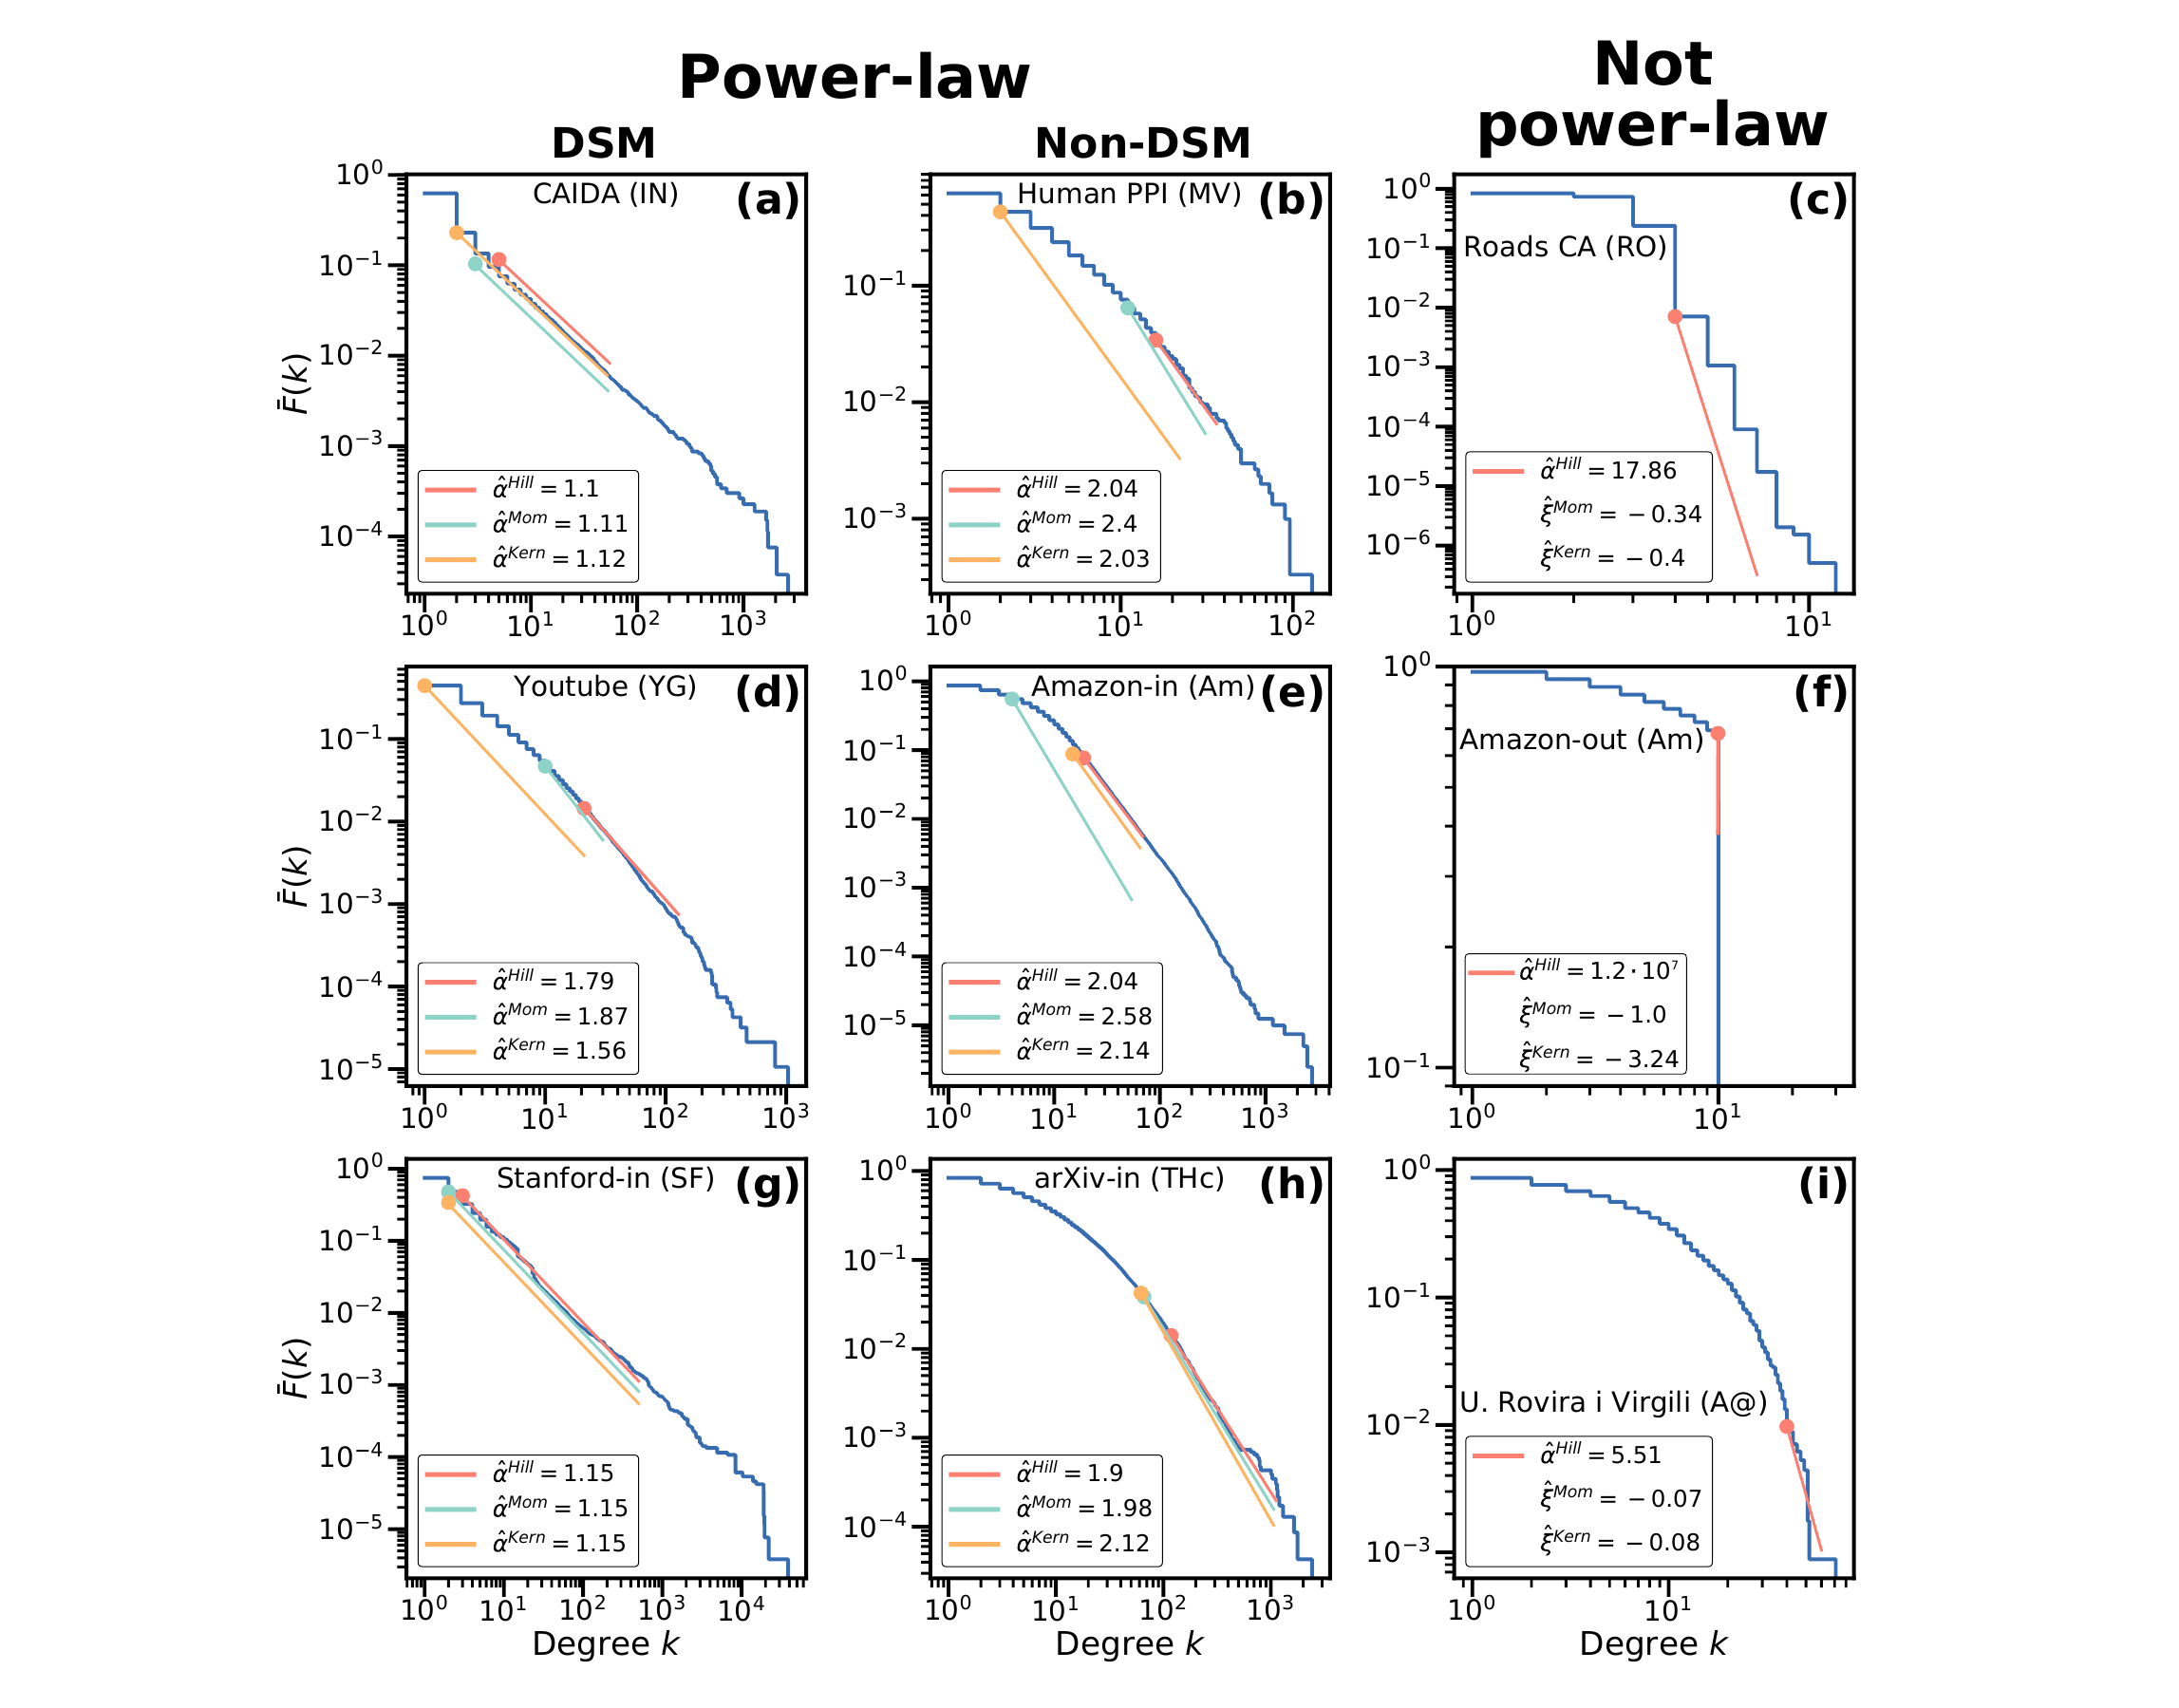
\includegraphics[width=0.92\textwidth]{figures/9_networks/Voitalov2019-degree-distributions.png}
\end{center}
Figure: Degree distributions of nine networks, plotted as the fraction of nodes with degree larger than $k$ (i.e., the complementary cumulative distribution $\bar F(k)$). Figure~2 of \hrefc{https://doi.org/10.1103/PhysRevResearch.1.033034}{Voitalov, van der Hoorn, van der Hofstad \& Krioukov, Phys.\ Rev.\ Research, 1, 033034 (2019)}, \hrefc{https://creativecommons.org/licenses/by/4.0/}{CC BY 4.0}.



\begin{enumerate}
\setcounter{enumi}{1}
\item Characteristic/average path length, $L$: how many hops one needs to go from one node to another, averaged over all the node pairs.
	\begin{itemize}
	\item $L = O(\log N)$ (as opposed to $L = O(N^{\alpha})$, $\alpha>0$) holds true in most empirical data unless the network is embedded in a space.
	\item $L = O(\log N)$ (or shorter) is often called \emph{small-world}.
		\begin{itemize}
		\item In network science, in most cases, small-world requires another property in addition to small $L$ (covered just below).
		\end{itemize}
	\end{itemize}
\end{enumerate}

\noindent\textbf{Example:} The square lattice yields $L=O(N^{1/2})$ and is not a realistic model for most social/biological/information/etc.\ networks. In general, a $d$-dimensional lattice yields $L=O(N^{1/d})$.

\begin{figure}[h]
\begin{center}
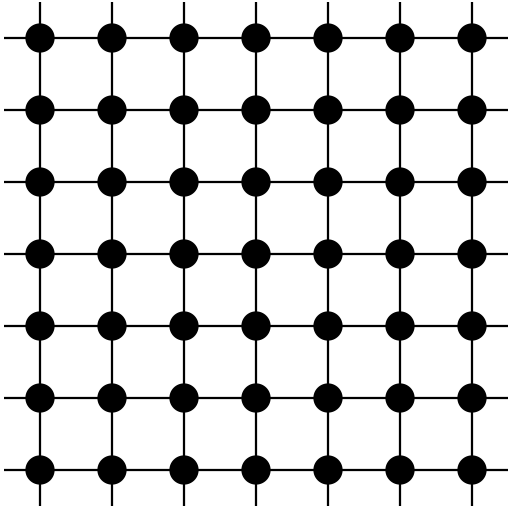
\includegraphics[width=0.5\textwidth]{figures/9_networks/square-lattice.png}
\caption{Square lattice.}
\end{center}
\end{figure}

\begin{figure}[h]
\begin{center}
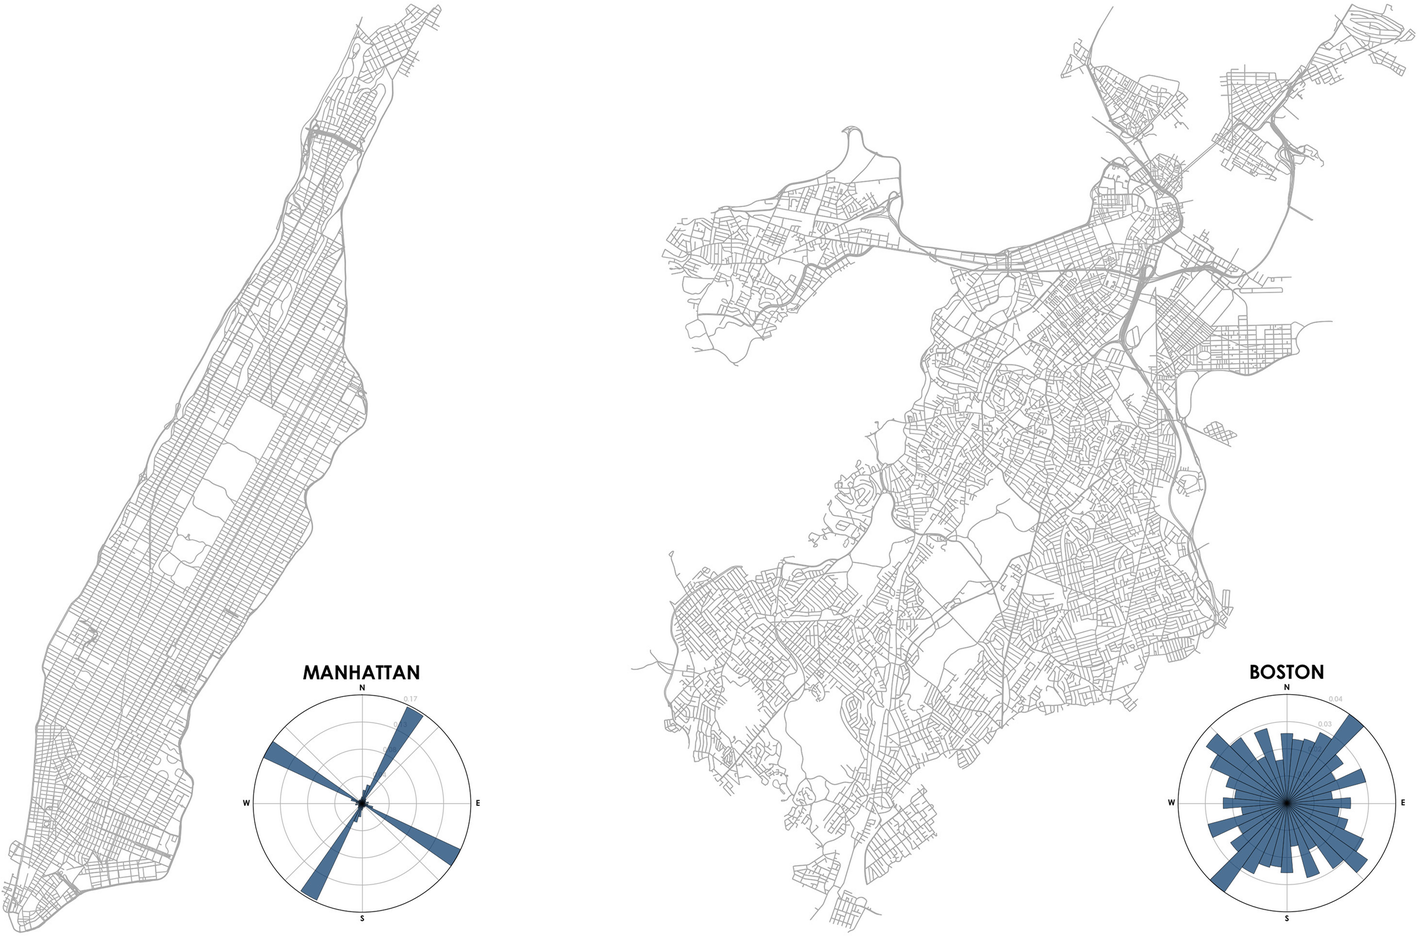
\includegraphics[width=0.95\textwidth]{figures/9_networks/Boeing2019-street-networks.png}
\caption{Street networks of Manhattan and Boston, two spatial networks. Figure~3 of \hrefc{https://doi.org/10.1007/s41109-019-0189-1}{Boeing, Applied Network Science, 4, 67 (2019)}, \hrefc{https://creativecommons.org/licenses/by/4.0/}{CC BY 4.0}.}
\end{center}
\end{figure}

% ============================================================================
% Clustering coefficient: commented out for the math-biology course (kept,
% not deleted, so it can be restored by removing the \iffalse ... \fi).
% ============================================================================
\iffalse
\begin{enumerate}
\setcounter{enumi}{2}
\item Clustering.
	\begin{itemize}
	\item In network science, clustering is used in the sense of triangle.
	\item Most empirical networks have high clustering, that is, they have many triangles.
	\end{itemize}
\end{enumerate}

\begin{itemize}
\item Clustering coefficient measures the abundance of triangles. One definition goes as follows:
\[
\begin{aligned}
C_i &= \text{ local clustering coefficient of the } i\text{th node }\\
&= \frac{(\text{number of triangles containing the } i \text{th node})}{\frac{k_i(k_i-1)}{2}},
\end{aligned}
\]
where $k_i$ is the degree of the $i$th node.
	\begin{itemize}
	\item Note that $0\le C_i \le 1$.
	\item (Global) clustering coefficient of the network: $C = \frac{1}{N} \sum_{i=1}^N C_i$.
	\end{itemize}
\end{itemize}

\noindent\textbf{Example:}

\begin{figure}[h]
\begin{center}
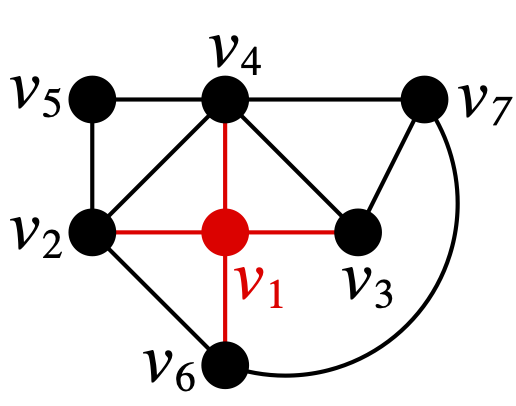
\includegraphics[width=0.3\textwidth]{figures/9_networks/c-calc-red.png}
\end{center}
\end{figure}

\[
\begin{aligned}
C_1 =& \frac{3}{4\times 3 / 2} = \frac{1}{2},\\
C_3 =& \frac{2}{3 \times 2 / 2} = \frac{2}{3},\\
C =& \frac{1}{7} \sum_{i=1}^7 C_i = \frac{8}{15}.
\end{aligned}
\]

\noindent\textbf{Exercise:} Calculate $C_5$ and $C_7$.


\begin{itemize}
\item We say that the network is small-world if it has a small $L$ and large $C$ (high clustering).
	\begin{itemize}
	\item But small/large relative to what? $\to$ Relative to randomized counterpart networks.
	\end{itemize}
\end{itemize}
\fi
% ============================================================================
% End of commented-out clustering coefficient block.
% ============================================================================

\begin{table}[h]
\begin{center}
\begin{tabular}{lcc}
\hline
Network & $L$ (actual) & $L$ (random) \\
\hline
Film actors & 3.65 & 2.99 \\
Power grid & 18.7 & 12.4 \\
\textit{C.\ elegans} & 2.65 & 2.25 \\
\hline
\end{tabular}
\caption{Average path length, $L$, of three empirical networks (``actual'') and of random networks with the same numbers of nodes and edges (``random''). Modified from Table~1 of \hrefc{https://doi.org/10.1038/30918}{Watts and Strogatz, Nature (1998)}: we show only the columns for $L$.}
\end{center}
\end{table}

\clearpage

\begin{enumerate}
\setcounter{enumi}{2}
\item Community is a densely connected subset of nodes, also called modules (but avoid the term \emph{cluster}, as it means triangle in network science).
\end{enumerate}

\begin{figure}[h]
\begin{center}
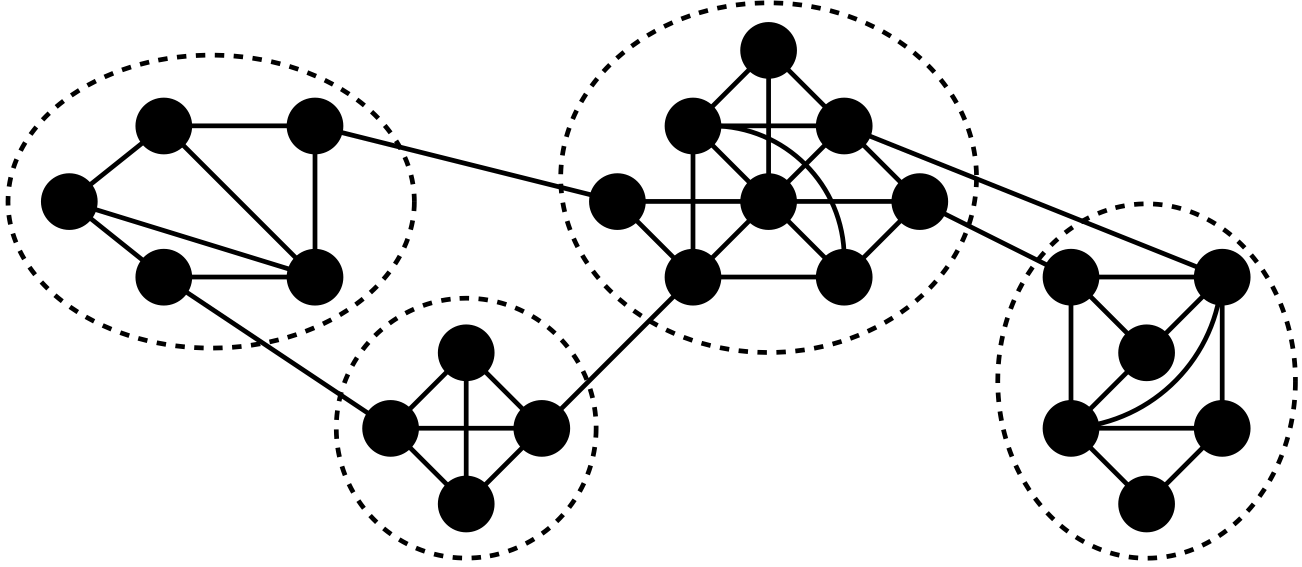
\includegraphics[width=0.6\textwidth]{figures/9_networks/comm.png}
\end{center}
\end{figure}

\begin{itemize}
\item Many networks have \emph{community} structure.
\end{itemize}

\begin{figure}[h]
\begin{center}
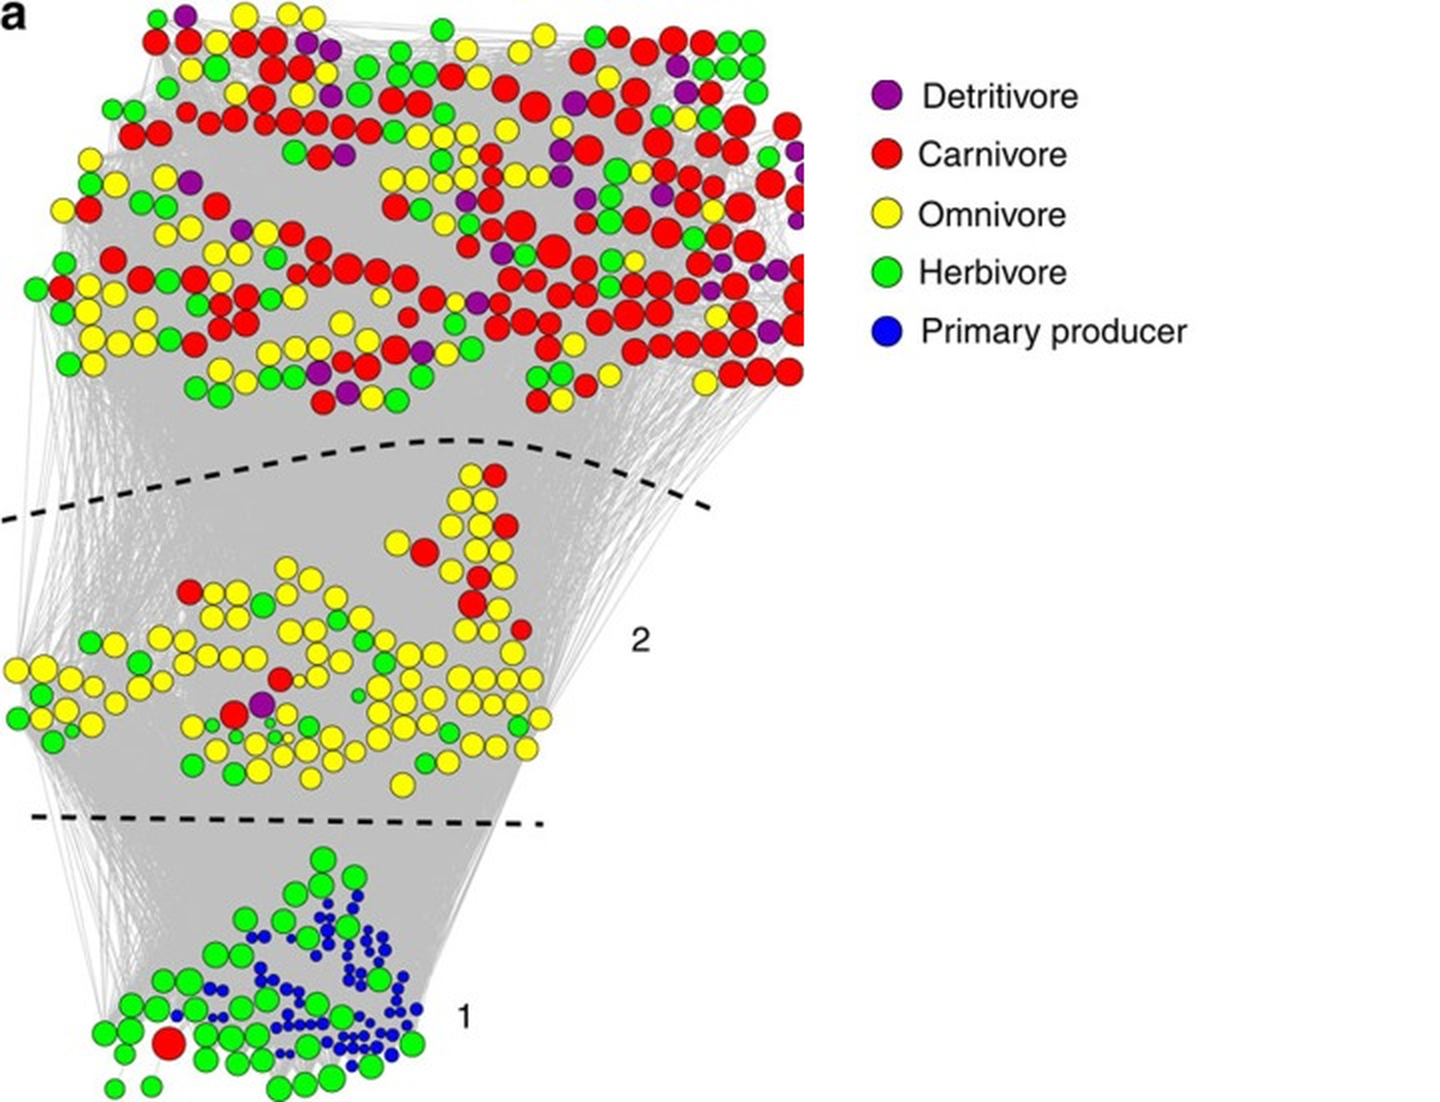
\includegraphics[width=0.78\textwidth]{figures/9_networks/NewmanClauset2016-foodweb.png}
\caption{Communities found in a food web of the Weddell Sea (Antarctica); an edge means that one species eats another. The algorithm divided the species into the three groups separated by the dashed lines, which turn out to correspond to trophic levels. Figure~3a (cropped) of \hrefc{https://doi.org/10.1038/ncomms11863}{Newman \& Clauset, Nature Communications, 7, 11863 (2016)}, \hrefc{https://creativecommons.org/licenses/by/4.0/}{CC BY 4.0}.}
\end{center}
\end{figure}

\begin{itemize}
\item How to find communities in given networks is a huge research field.
	\begin{itemize}
	\item E.g., modularity maximization by \hrefc{https://websites.umich.edu/~mejn/}{Mark E.~J.~Newman} at U-M Physics / Complex Systems, stochastic block models, information-theoretic approaches, etc.
	\item There is no single standard/algorithm.
	\end{itemize}
\end{itemize}

\subsection*{Networks are modeling for complex system data}

\begin{itemize}
\item Networks themselves are a model of complex system data.
	\begin{itemize}
	\item Transportation networks (such as airports), social networks, stocks, international relations, the Internet, the WWW, citations among research articles, $\ldots$
	\item Biology, medicine: food webs, the brain, gene regulation, drug--drug relations, communication among MDs, $\ldots$
	\item Analysis of network \emph{structure} leads to useful knowledge. E.g., PageRank identifying key persons, disease-gene discovery through \emph{gene module} analysis.
	\end{itemize}
\end{itemize}

% ============================================================================
% New math-biology / medicine sections (for the MATH 463 version).
% ============================================================================

\subsection*{Network biology and network medicine}

\begin{itemize}
\item Two closely related subfields of network science applied to the life sciences:
	\begin{itemize}
	\item \textbf{Network biology}: model molecular systems (genes, proteins, metabolites, $\ldots$) as networks and study their structure and function.\\
	Review: \hrefc{https://doi.org/10.1038/nrg1272}{Barab\'asi and Oltvai, Nature Reviews Genetics (2004)}.
	\item \textbf{Network medicine}: apply network science to human disease, e.g., disease genes, comorbidity, drug targets.\\
	Review: \hrefc{https://doi.org/10.1038/nrg2918}{Barab\'asi, Gulbahce and Loscalzo, Nature Reviews Genetics (2011)}.\\
	Book: \hrefc{https://www.hup.harvard.edu/books/9780674436534}{Network Medicine (2017)}.
	\end{itemize}
\item Why networks? The traditional ``one-gene, one-disease'' reductionist view is often too simple.
	\begin{itemize}
	\item Most clinical phenotypes are biologically heterogeneous (``complex diseases'').
	\item A disease may disrupt an \emph{interaction} between molecules, rather than the expression of a single gene in isolation.
	\item So we want to understand and exploit interactions among molecules/genes: a \emph{systems} (network) approach.
	\end{itemize}
\end{itemize}

\subsection*{Gene modules}

\begin{itemize}
\item \textbf{Gene networks}
	\begin{itemize}
	\item Nodes are genes.
	\item \emph{regulation}: the product of one gene (e.g., a transcription factor) controls the expression (i.e.,\,amount of RNA produced) of another gene. This is naturally a \emph{directed} edge.
		\begin{itemize}
		\item Gene-regulatory networks (GRNs)
		\end{itemize}
	\item \emph{co-expression}: two genes are expressed together (their expression levels are correlated across samples/conditions). This is an \emph{undirected} edge.
	\end{itemize}
	\item \textbf{Q:} Which network is easier to measure and why?
\end{itemize}

\begin{center}
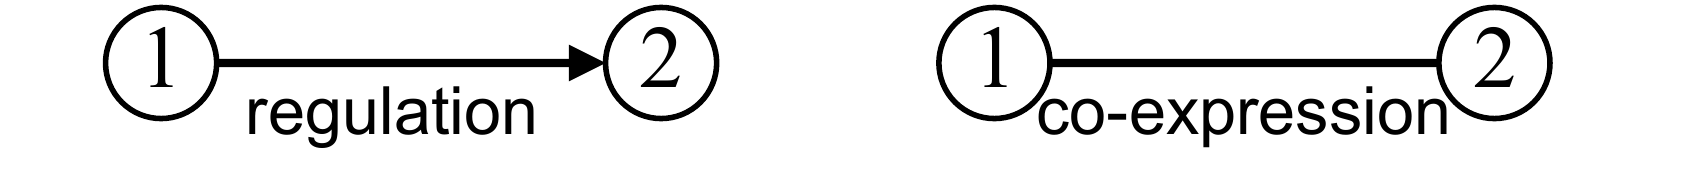
\includegraphics[width=0.85\textwidth]{figures/9_networks/gene-network-edges.png}\\
Two common types of edge in a gene network.
\end{center}

\begin{figure}[h]
\begin{center}
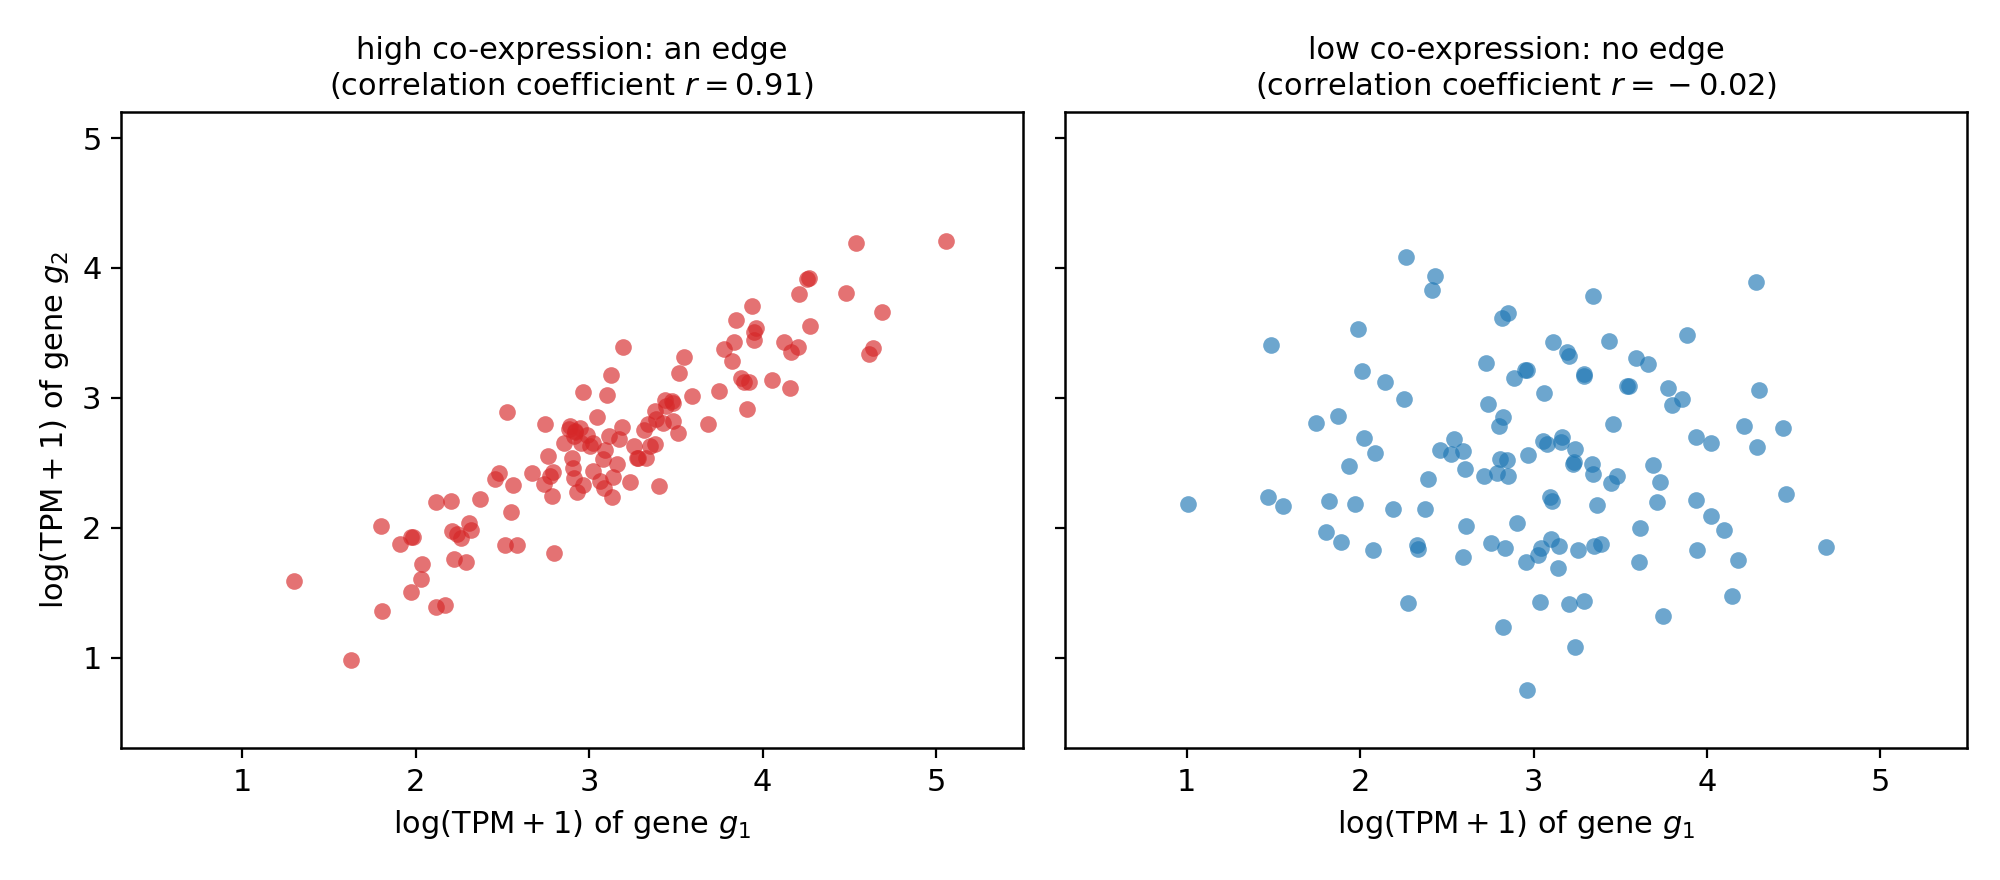
\includegraphics[width=0.95\textwidth]{figures/9_networks/coexpression.png}
\caption{What a co-expression edge means. Each dot represents one sample (e.g., one tissue sample or one patient). TPM: transcripts per million. The data here are made up for illustration.}
\end{center}
\end{figure}

\begin{itemize}
\item \textbf{Gene module $\approx$ network community.}
	\begin{itemize}
	\item A \emph{gene module} is a group of genes that are densely connected among themselves (co-regulated, co-expressed, or physically interacting).
	\item This is basically a \emph{community} in a network.
	\item Genes in a gene module often share a biological function. 
	\end{itemize}
\item \textbf{Why useful?} Genes associated with the same disease tend to be in the same module (the disease module hypothesis; guilt by association). So, if some members of a module are already known disease genes, the other members become strong \emph{candidates}. This narrows down the search for disease-related genes (instead of testing all $\sim$20{,}000 human genes one by one).
\item \textbf{Q:} What would be guilt-by-association inference in human social networks?
	\begin{itemize}
	\item Note: Human social networks almost always have community structure.
	\end{itemize}
\end{itemize}

\begin{figure}[h]
\begin{center}
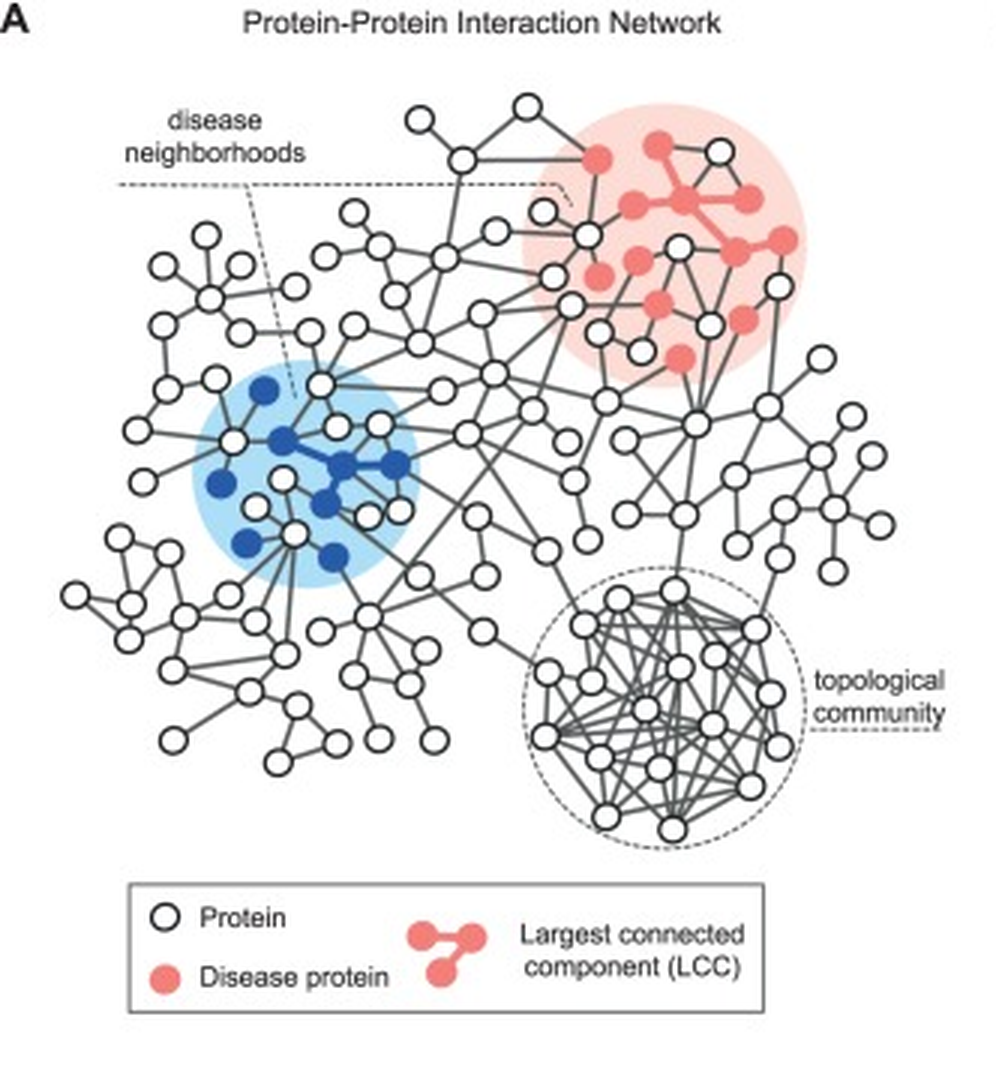
\includegraphics[width=0.62\textwidth]{figures/9_networks/Ghiassian2015-disease-module.png}
\caption{Disease modules in a protein-protein interaction network. The two shaded neighborhoods are the modules of two different diseases. The dashed circle shows a densely connected community that is not a disease module. Figure~1A (cropped) of \hrefc{https://doi.org/10.1371/journal.pcbi.1004120}{Ghiassian, Menche \& Barab\'asi, PLOS Computational Biology, 11, e1004120 (2015)}, \hrefc{https://creativecommons.org/licenses/by/4.0/}{CC BY 4.0}.}
\end{center}
\end{figure}

\clearpage

\subsection*{Obesity spreads through social networks}

\begin{itemize}
\item Nicholas Christakis (Harvard $\to$ Yale) and James Fowler (UCSD) used the Framingham Heart Study data (thousands of people whose social ties (edges) and health were tracked over decades) to argue that health states and behaviors spread from person to person in social networks.
\item Obesity spreads through social networks: a person's chance of becoming obese increases when a friend becomes obese (\hrefc{https://doi.org/10.1056/NEJMsa066082}{Christakis \& Fowler, New England Journal of Medicine (2007)}).
	\begin{itemize}
	\item \textbf{Q:} Is obesity biologically contagious like flu or COVID-19?
	\item \textbf{Q:} Homophily is present in almost any social networks. Isn't it that obese people tend to become friends with other obese people, and lean people do the same? What data would we need to distinguish homophily from contagion?
\vspace{3cm}
	\item Where is math? --- A backstory.
	\end{itemize}
\end{itemize}

\begin{figure}[h]
\begin{center}
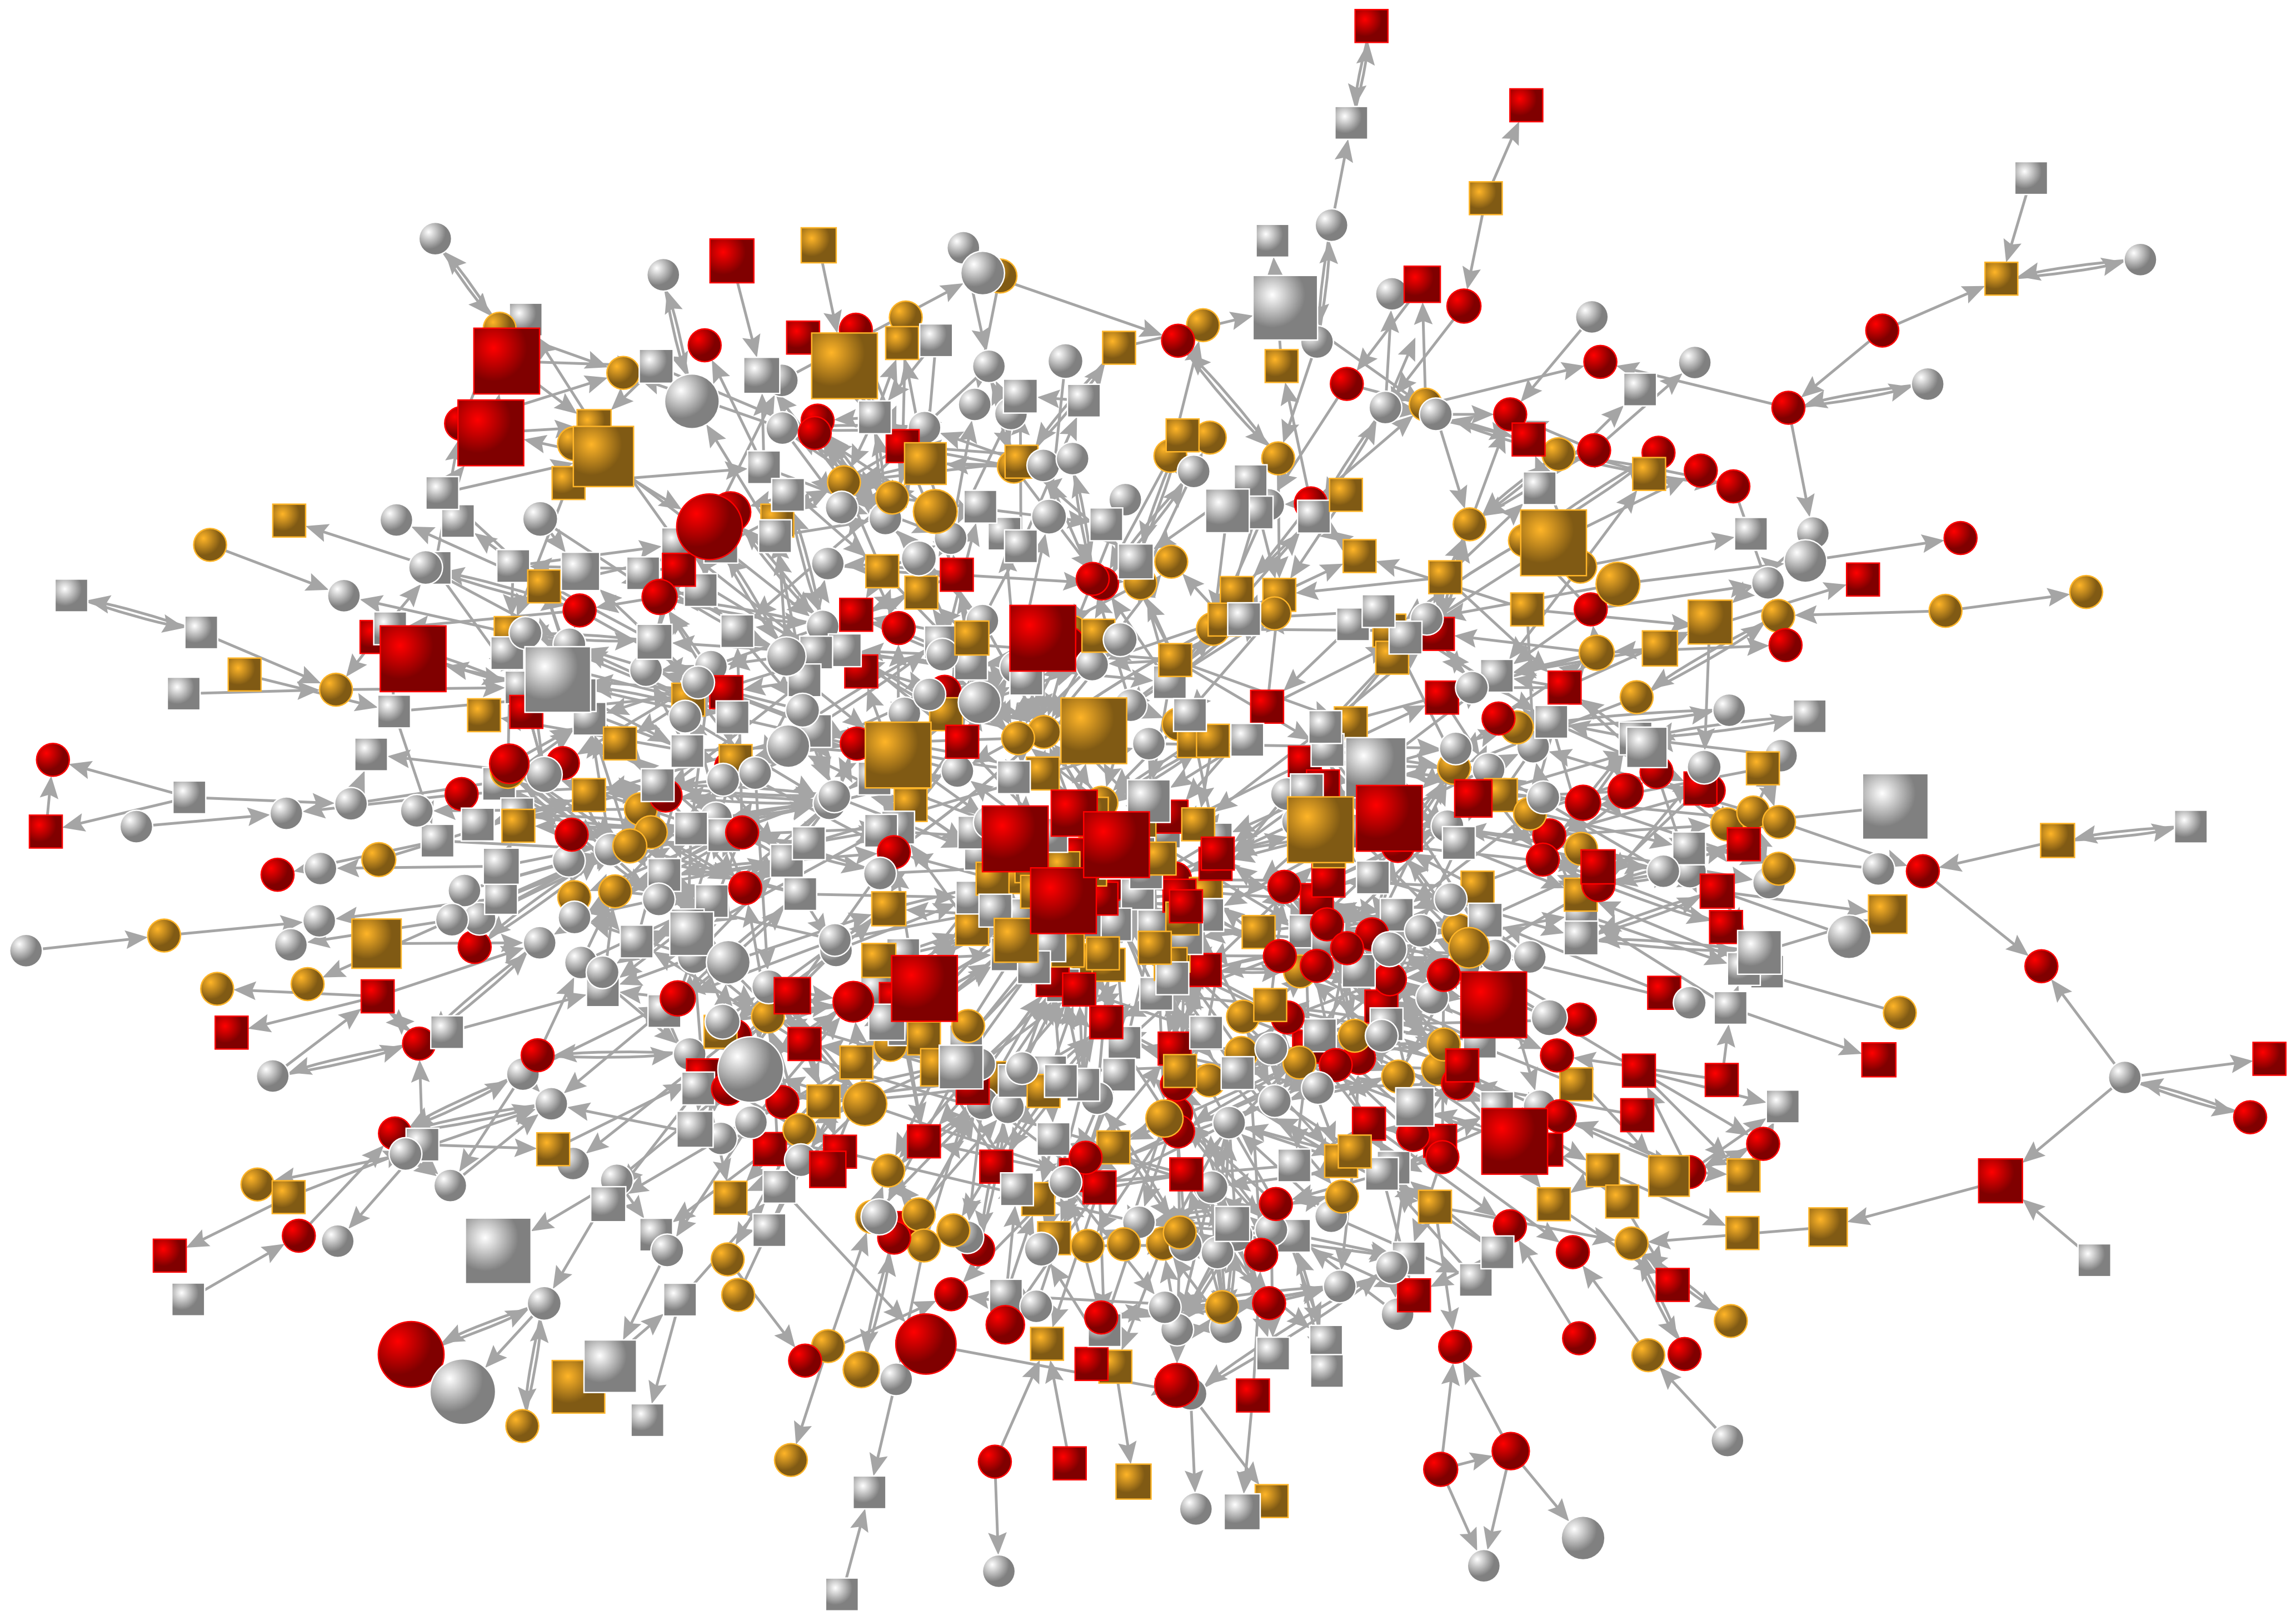
\includegraphics[width=0.9\textwidth]{figures/9_networks/Mednick2010-sleep-network.png}
\caption{A friendship network of 800 students at a US school. Node color shows nightly sleep (red: 6 hours or less; orange: 7 hours; white: 8 hours or more). Node size shows how often the student uses marijuana (smallest: never; largest: at least daily). Circles are female students, and squares are male students. An arrow points from a student to a friend whom the student named. Both short sleep and drug use cluster in the network. Figure~1 of \hrefc{https://doi.org/10.1371/journal.pone.0009775}{Mednick, Christakis \& Fowler, PLoS ONE, 5, e9775 (2010)}, licensed under \hrefc{https://creativecommons.org/licenses/by/4.0/}{CC BY 4.0}.}
\label{fig:sleep-network}
\end{center}
\end{figure}

\begin{itemize}
\item Also ``contagious'' are, e.g.:
	\begin{itemize}
	\item happiness: \hrefc{https://doi.org/10.1136/bmj.a2338}{Fowler \& Christakis, BMJ (2008)}
	\item depression: \hrefc{https://doi.org/10.1038/mp.2010.13}{Rosenquist et al., Molecular Psychiatry (2011)}
	\item smoking: \hrefc{https://doi.org/10.1056/NEJMsa0706154}{Christakis \& Fowler, New Eng J Med (2008)}
	\item loneliness: \hrefc{https://doi.org/10.1037/a0016076}{Cacioppo et al., J Pers and Soc Psychol (2009)}
	\item sleep loss and drug use: \hrefc{https://doi.org/10.1371/journal.pone.0009775}{Mednick, Christakis \& Fowler, PLoS ONE (2010)}
	\end{itemize}
\item Popular-science book: \hrefc{https://www.amazon.com/Connected-Surprising-Networks-Friends-Everything/dp/0316036137}{Connected, Christakis \& Fowler (2009)}.
\end{itemize}

\clearpage

\subsection*{Disease networks}

\begin{itemize}
\item In a \emph{disease network}, the nodes are diseases, and an edge connects two diseases that are related in some way. Different notions of ``related'' give different disease networks.
\item \textbf{Motivation:} Comorbidity (a.k.a.\ multimorbidity) is the simultaneous occurrence of several diseases in the same individual. A shared gene or molecular mechanism can trigger several diseases. Disease networks help anticipate how patients progress from one illness to another.
\item \textbf{Human disease network} (\hrefc{https://doi.org/10.1073/pnas.0701361104}{Goh et al., PNAS (2007)}): connect two diseases if they share at least one associated gene. The resulting ``diseasome'' shows that diseases of the same class tend to cluster together.
\item \textbf{Phenotypic disease network} (\hrefc{https://doi.org/10.1371/journal.pcbi.1000353}{Hidalgo et al., PLoS Comput.\ Biol.\ (2009)}): connect two diseases if they occur in the same patients more often than expected by chance (comorbidity), measured from the medical records of patients.
\end{itemize}

\begin{figure}[h]
\begin{center}
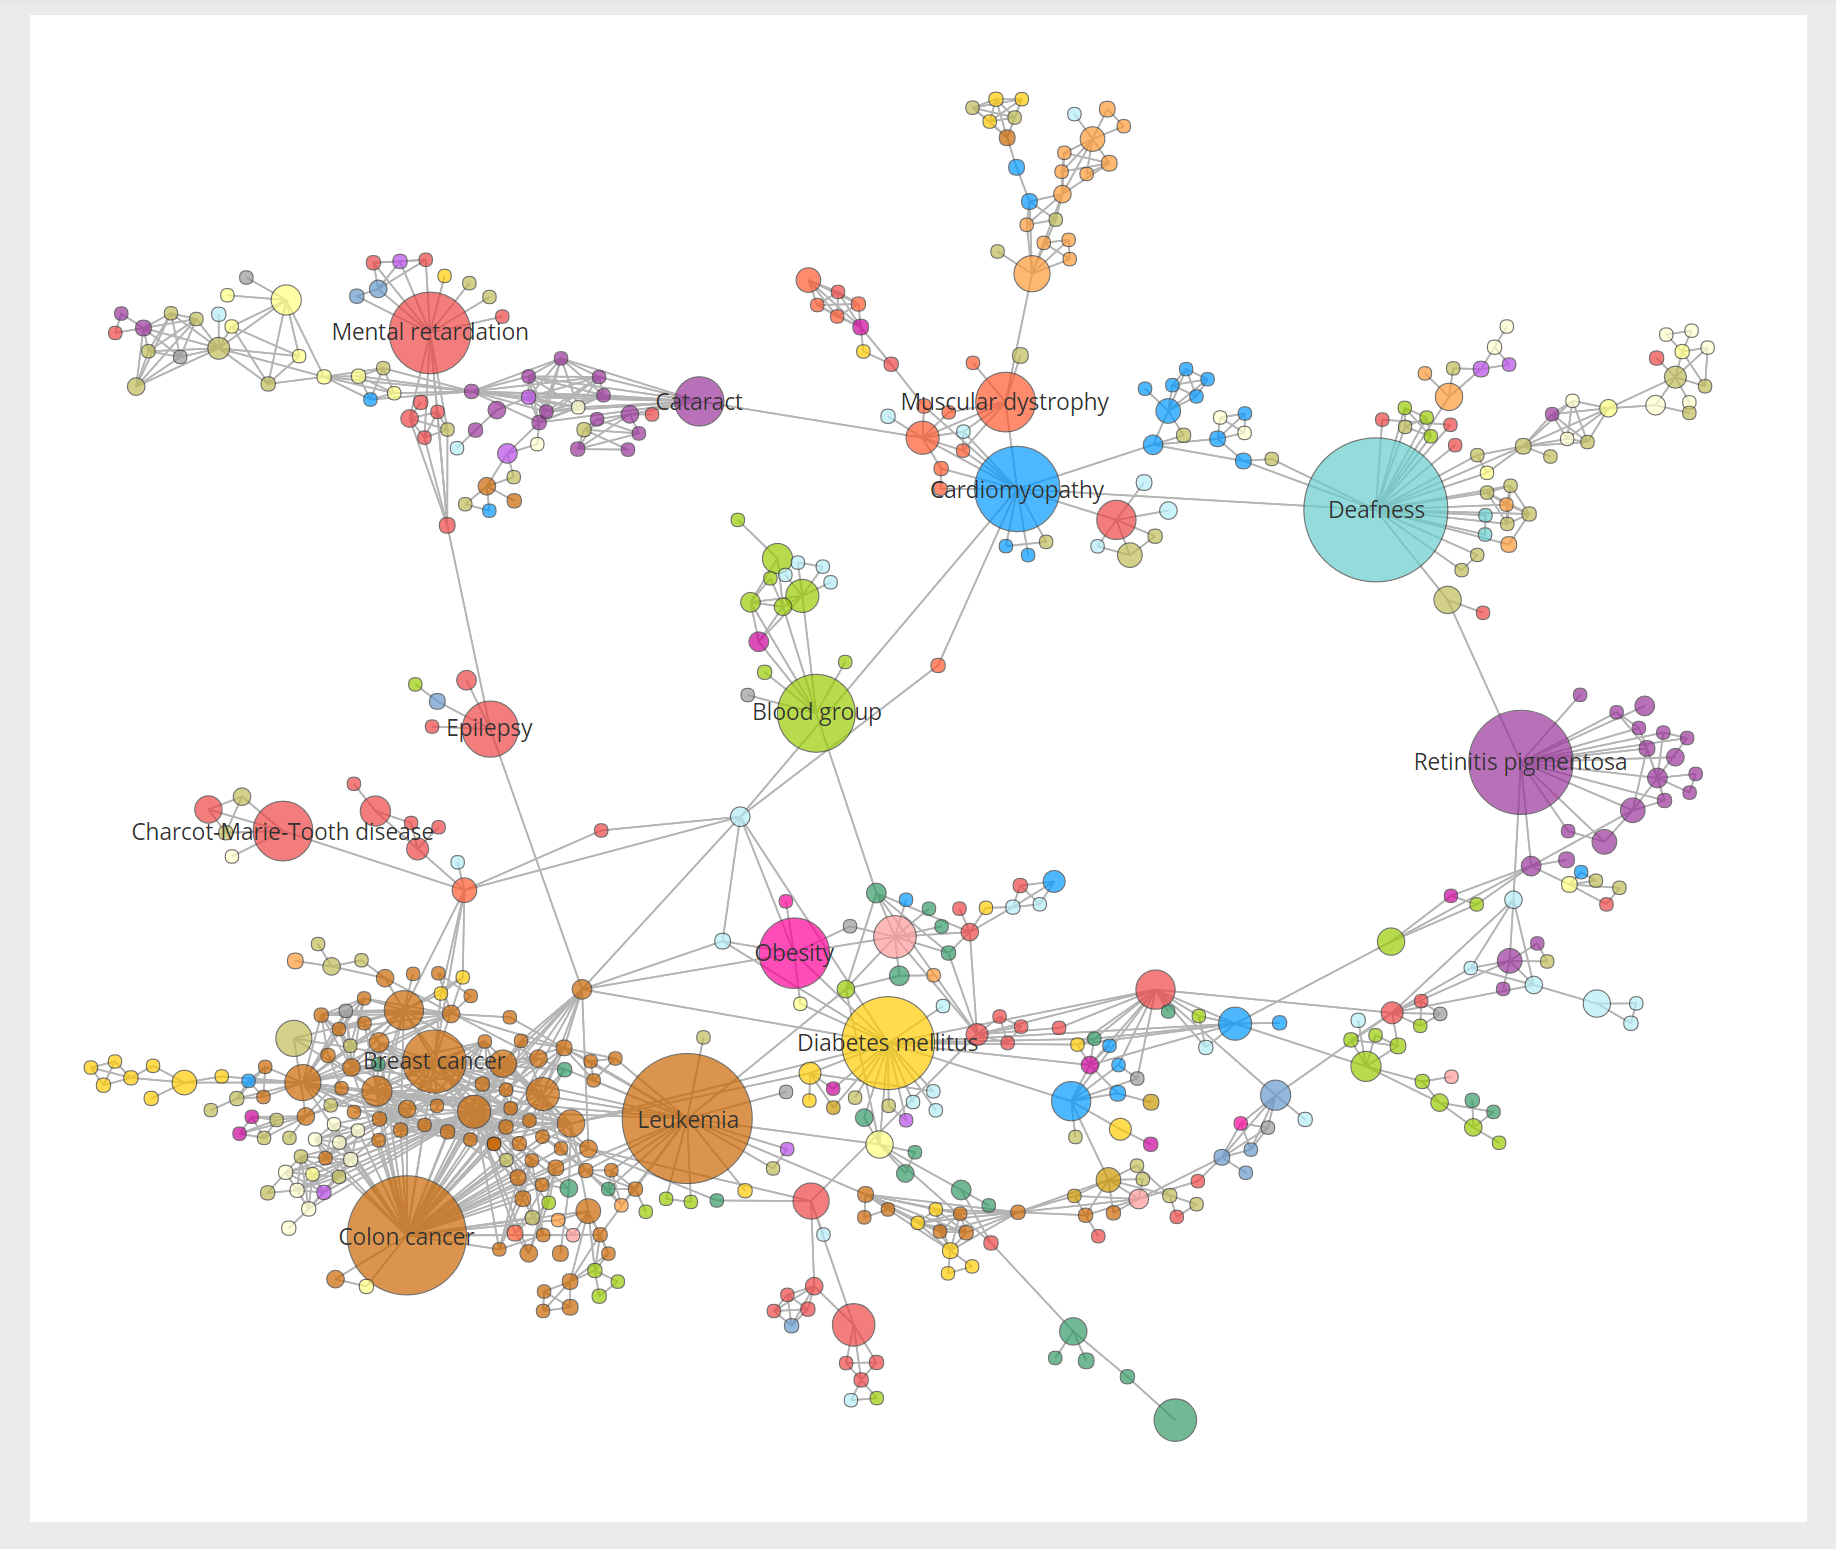
\includegraphics[width=0.5\textwidth]{figures/9_networks/Commons-HDN.png}\\[1ex]
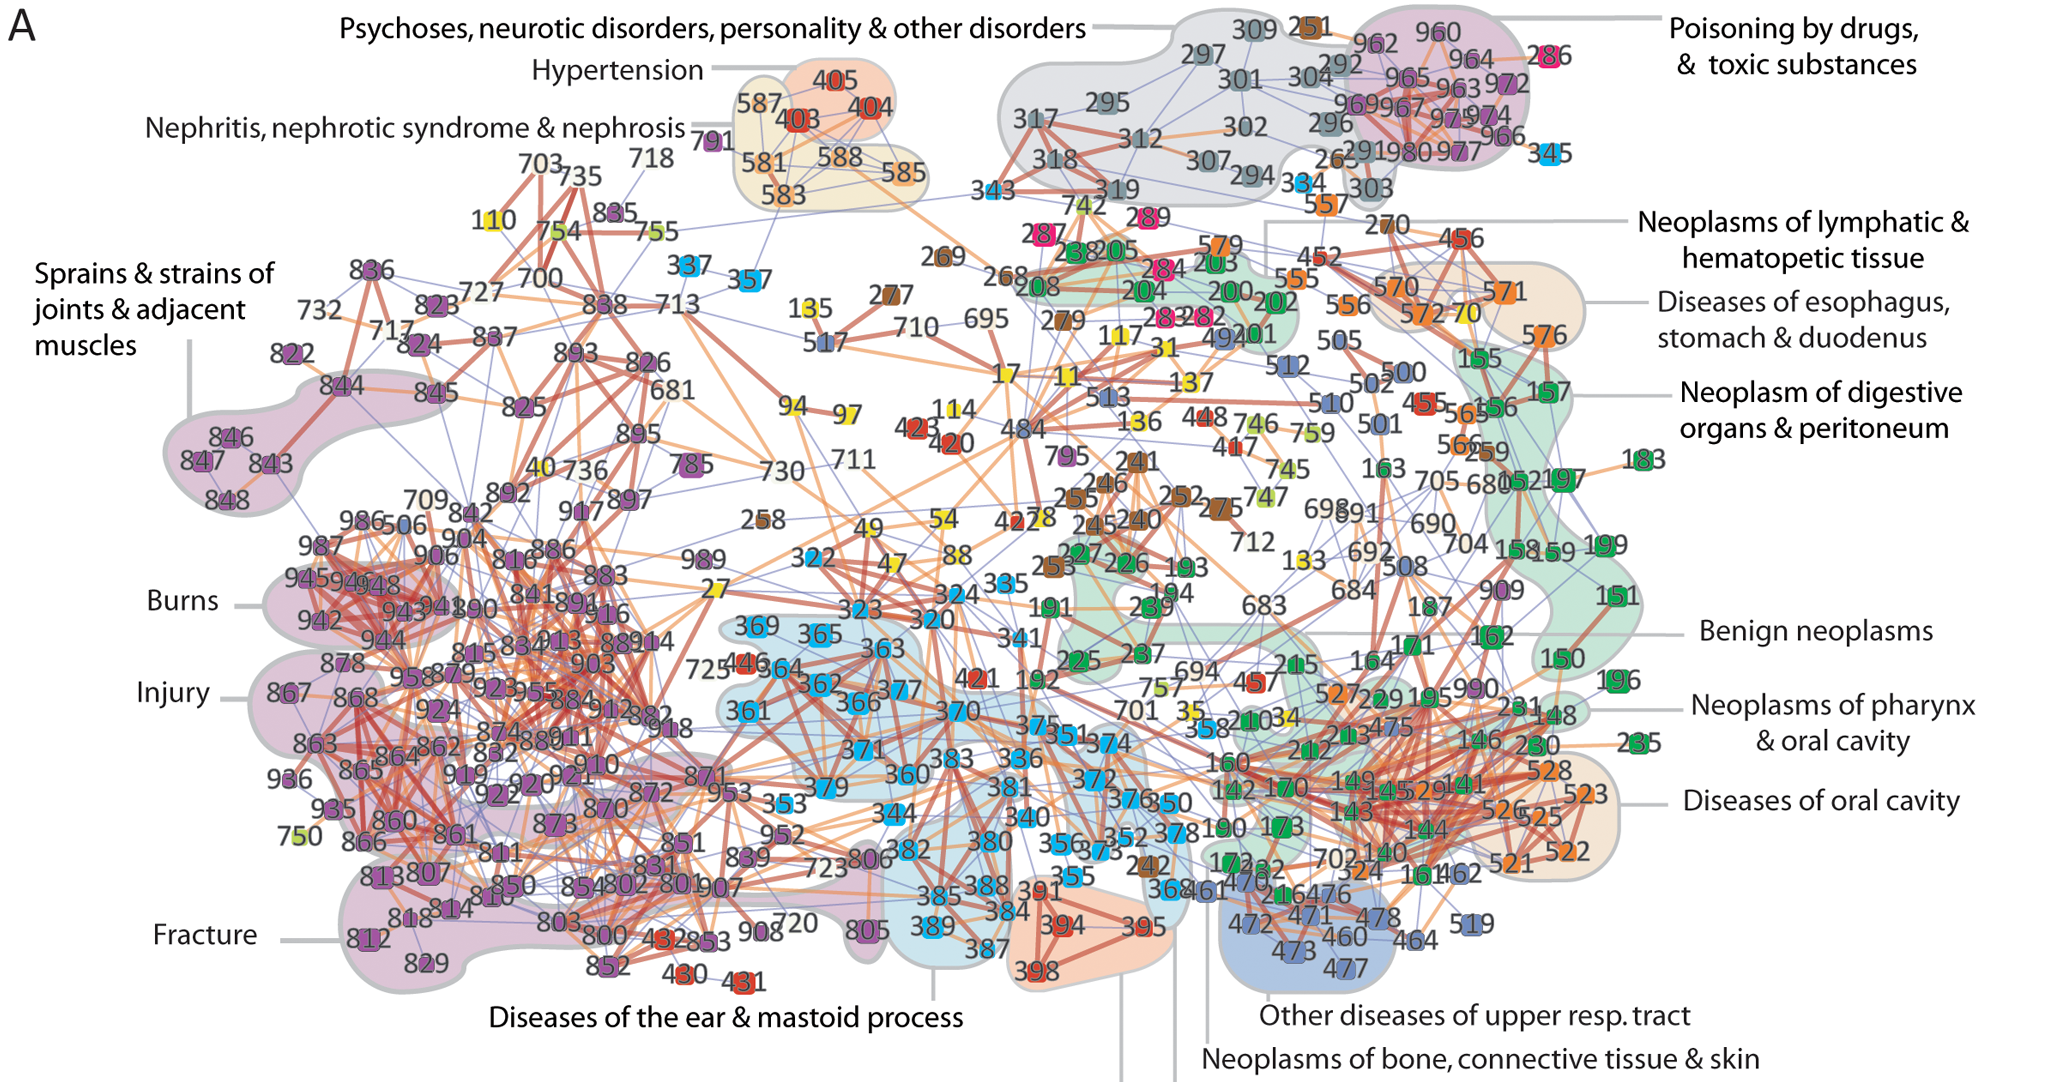
\includegraphics[width=0.8\textwidth]{figures/9_networks/Hidalgo2009-pdn.png}
\caption{Disease networks. Top: human disease network; two diseases are connected if they share a gene. \hrefc{https://commons.wikimedia.org/wiki/File:HDN.png}{``HDN.png'' by Empetrisor, Wikimedia Commons}, drawn from the data of \hrefc{https://doi.org/10.1073/pnas.0701361104}{Goh et al., PNAS (2007)}, licensed under \hrefc{https://creativecommons.org/licenses/by-sa/4.0/}{CC BY-SA 4.0}. Bottom: phenotypic disease network; two diseases are connected if they are comorbid. Each number is an ICD-9 disease code, and the node color shows the disease category. Figure~2A (cropped) of \hrefc{https://doi.org/10.1371/journal.pcbi.1000353}{Hidalgo, Blumm, Barab\'asi \& Christakis, PLoS Comput.\ Biol., 5, e1000353 (2009)}, licensed under \hrefc{https://creativecommons.org/licenses/by/4.0/}{CC BY 4.0}.}
\end{center}
\end{figure}

\clearpage

\begin{itemize}
\item Other ways to define an edge between two diseases:
	\begin{itemize}
	\item \emph{metabolic} disease network: two diseases are linked if their associated metabolic reactions are adjacent, i.e., share a metabolite that is not too common (\hrefc{https://doi.org/10.1073/pnas.0802208105}{Lee et al., PNAS (2008)}).
	\end{itemize}
\end{itemize}

% ============================================================================
% End of new math-biology / medicine sections.
% ============================================================================

\subsection*{Friendship paradox}

\begin{itemize}
\item ``Your friend has more friends than you do (on average).''
	\begin{itemize}
	\item By \hrefc{https://www.doi.org/10.1086/229693}{Feld, American Journal of Sociology (1991)}.
	\item This is a purely mathematical phenomenon.
	\item Always so unless every node has the same degree.
	\item Many surprises in network science originate from this.
	\end{itemize}
\item Preparation:
	\begin{itemize}
	\item $p(k)$: degree distribution.
		\begin{itemize}
		\item \textbf{Exercise:} In the following network, $p(1)$? $p(2)$?
		\end{itemize}
	\item Average degree: $\langle k\rangle = \sum_k k\, p(k)$.
	\end{itemize}
\end{itemize}

\begin{center}
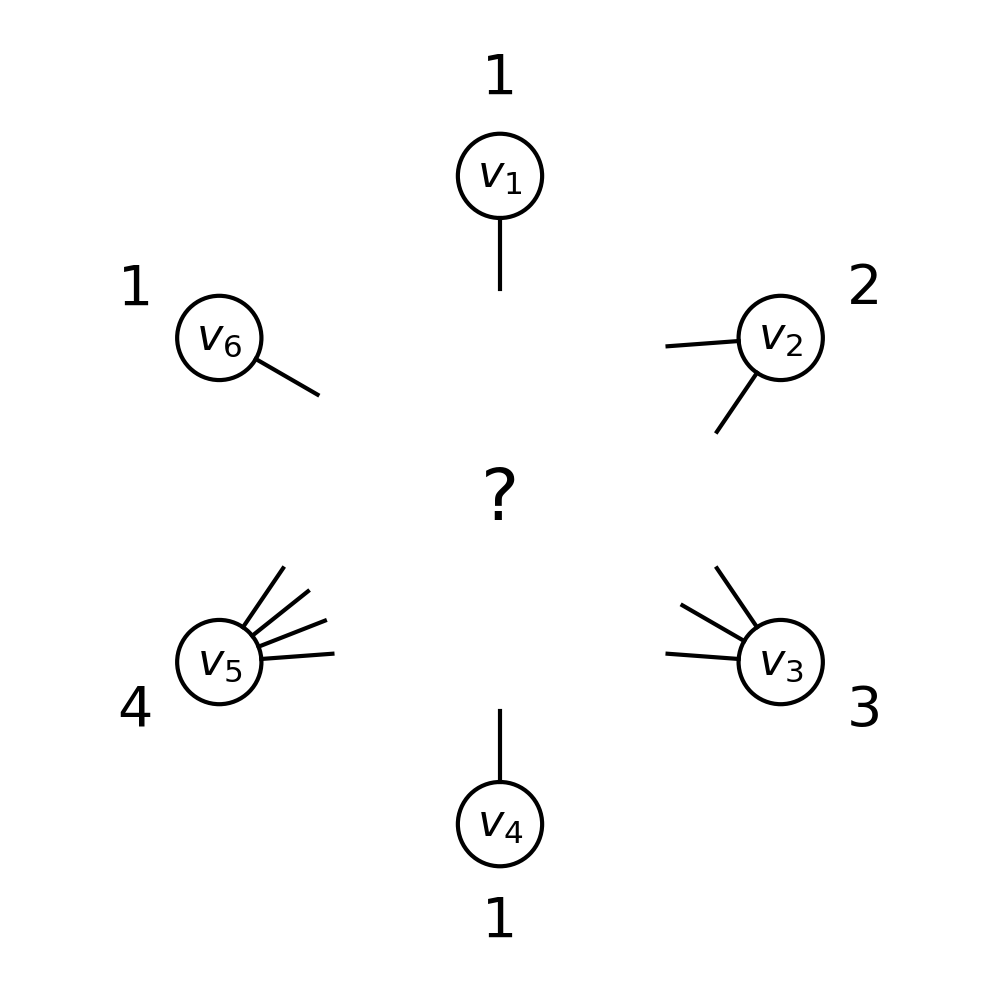
\includegraphics[width=0.4\textwidth]{figures/9_networks/friendship-paradox-stubs.png}\\
The numbers represent the node's degree.
\end{center}


\begin{itemize}
\item This network has $N=6$ nodes.
\item Let's pretend not to know the actual edges.
\[ \langle k \rangle = \frac{1}{6} (1+2+3+1+4+1) = 2. \]
\end{itemize}

\noindent\textbf{Question:} $p(v_1\text{'s neighbor is } v_4)$?\\
\textbf{A:} Not $1/5$. But
\[ p(v_1\text{'s neighbor is } v_4) = \frac{1}{2+3+1+4+1} = \frac{1}{11}, \]
which is smaller than $\frac{1}{5}$!

\medskip
\noindent\textbf{Question:} $p(v_1\text{'s neighbor is } v_5)$?\\
\textbf{A:} $\frac{4}{2+3+1+4+1} = \frac{4}{11}$, which is larger than $\frac{1}{5}$.

\begin{itemize}
\item So, \emph{hubs} (i.e., high-degree nodes) are more likely to be selected as a neighbor (of somebody).
\item This is an example of biased sampling.
\end{itemize}

\noindent\textbf{Question:} $\langle k \rangle_{v_1\text{'s neighbor}}$?\\
\textbf{A:} It is not $\frac{2+3+1+4+1}{5} = \frac{11}{5} = 2.2$.
\[ \frac{2}{11} \times 2 + \frac{3}{11} \times 3 + \frac{1}{11} \times 1 + \frac{4}{11} \times 4 + \frac{1}{11} \times 1 = \frac{31}{11} \approx 2.82 > 2.2. \]

\begin{itemize}
\item A node with degree $k$ appears $k$ times when calculating $p(\text{being a neighbor of a node})$.
\item So, the average number of friends of a friend (i.e.\ average degree of a neighbor):
{\small
\[ = \frac{(1 \times 1+ 2 \times 2 + 3 \times 3 + 1 \times 1+ 4 \times 4 + 1 \times 1)}{(1+2+3+1+4+1)} \approx 2.67 > 2 = \langle k\rangle. \]
}
In general,
\[ \langle k\rangle_{\text{neighbor}} = \sum_k k \times \frac{kp(k)}{\sum_{k^{\prime}} k^{\prime} p(k^{\prime})} = \frac{\langle k^2\rangle}{\langle k\rangle}. \]
\item Since
\[ \sigma^2 = \langle (x-\langle x\rangle)^2 \rangle = \langle x^2 \rangle - \langle x \rangle^2 \ge 0, \]
we have $\frac{\langle k^2\rangle}{\langle k\rangle} \ge \langle k\rangle$, and $=$ holds iff $\sigma^2 = 0$ (i.e.\ \emph{regular graphs}, where all nodes have the same degree $\langle k\rangle$).
\end{itemize}

\noindent\textbf{Example 1:} Erd\H{o}s--R\'enyi (ER) random graph.

\begin{itemize}
\item $N$ nodes.
\item Each pair of nodes is connected independently with probability $p$.
\end{itemize}

\begin{figure}[h]
\begin{center}
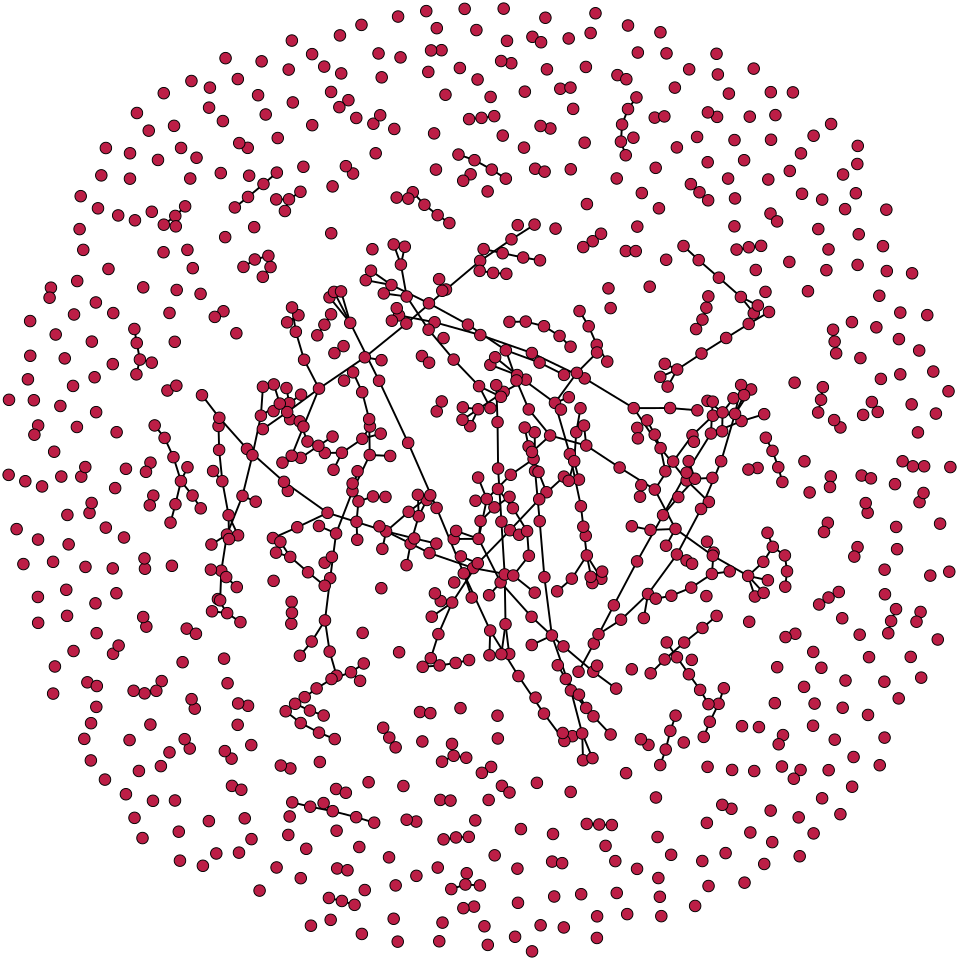
\includegraphics[width=0.75\textwidth]{figures/9_networks/Critical_1000-ER-wikipedia.png}
\caption{A network generated by the ER random graph model with 1000 nodes at the critical edge probability, $p=1/(N-1)$. \hrefc{https://commons.wikimedia.org/wiki/File:Critical_1000-vertex_Erd\%C5\%91s\%E2\%80\%93R\%C3\%A9nyi\%E2\%80\%93Gilbert_graph.svg}{``Critical 1000-vertex Erd\H{o}s--R\'enyi--Gilbert graph'' by David Eppstein, Wikimedia Commons}, released into the public domain under \hrefc{https://creativecommons.org/publicdomain/zero/1.0/}{CC0 1.0}.}
\end{center}
\end{figure}

\begin{itemize}
\item For this network, it is known that the degree distribution is a binomial distribution, or
\[ p(k) = \frac{(N-1)!}{k!(N-1-k)!} p^k (1-p)^{N-1-k}. \]
\item $\langle k \rangle = (N-1)p$.
\item Variance $= \langle k^2 \rangle - \langle k \rangle^2 = (N-1)p(1-p)$. So,
\[
\begin{aligned}
\langle k\rangle_{\text{neighbor}} &= \frac{\langle k^2\rangle}{\langle k\rangle} =
\frac{\text{Variance} + \langle k\rangle^2}{\langle k\rangle}\\
&= \frac{(N-1)p(1-p) + \left[(N-1)p\right]^2}{(N-1)p}\\
&= 1-p + (N-1)p = 1-p + \langle k\rangle.
\end{aligned}
\]
\item When $N$ is large and $p$ is small (which is a usual assumption for the ER random graph), we get
\[ \langle k\rangle_{\text{neighbor}} \approx \langle k\rangle + 1. \]
So, your average friend has one more friend than you do.
\end{itemize}

\noindent\textbf{Example 2:} Scale-free network.
\begin{itemize}
\item $p(k) = \mathcal{N} k^{-\gamma}$, where $\mathcal{N}$ is a normalization constant.
\item To get analytical insights, let's presume that $k$ is a continuous variable.
\item By requiring
\[ \int^{\infty}_{k_{\min}}p(k)\text{d}k = \frac{\mathcal{N}}{1-\gamma}\left[k^{-\gamma+1}\right]^{\infty}_{k_{\min}} = 1, \]
we get
\[ \mathcal{N}=(\gamma-1)k_{\min}^{\gamma-1}. \]
Using this,
\[
\begin{aligned}
\langle k\rangle = \int^{\infty}_{k_{\min}} kp(k)\text{d}k
=& \mathcal{N} \int^{\infty}_{k_{\min}}k^{-\gamma+1}\text{d}k\\
=& \frac{(\gamma-1)k_{\min}^{\gamma-1}}{2-\gamma}
\left[k^{-\gamma+2}\right]^{\infty}_{k_{\min}} = \frac{\gamma-1}{\gamma-2}k_{\min},
\end{aligned}
\]
and
\[
\begin{aligned}
\langle k^2\rangle = \int^{\infty}_{k_{\min}}k^2\times \mathcal{N} k^{-\gamma}\text{d}k
=& \frac{(\gamma-1)k_{\min}^{\gamma-1}}
{3-\gamma} \left[k^{-\gamma+3} \right]^{\infty}_{k_{\min}}\\
=& \frac{\gamma-1}{\gamma-3} k_{\min}^2.
\end{aligned}
\]
\item We assumed $\gamma > 3$.
\[ \langle k\rangle_{\text{neighbor}} = \frac{\langle k^2\rangle}{\langle k\rangle} =
\frac{\frac{\gamma-1}{\gamma-3}k_{\min}^2} {\frac{\gamma-1}{\gamma-2}k_{\min}} = \frac{\gamma-2}{\gamma-3} k_{\min}
= \frac{(\gamma-2)^2}{(\gamma-1)(\gamma-3)}\langle k\rangle. \]
This is much larger than $\langle k\rangle$ if $\gamma \to 3$.
\end{itemize}

\subsection*{Disease spreading on complex networks}

\begin{itemize}
\item We did the SIS model on networks.
\end{itemize}

\begin{figure}[h]
\begin{center}
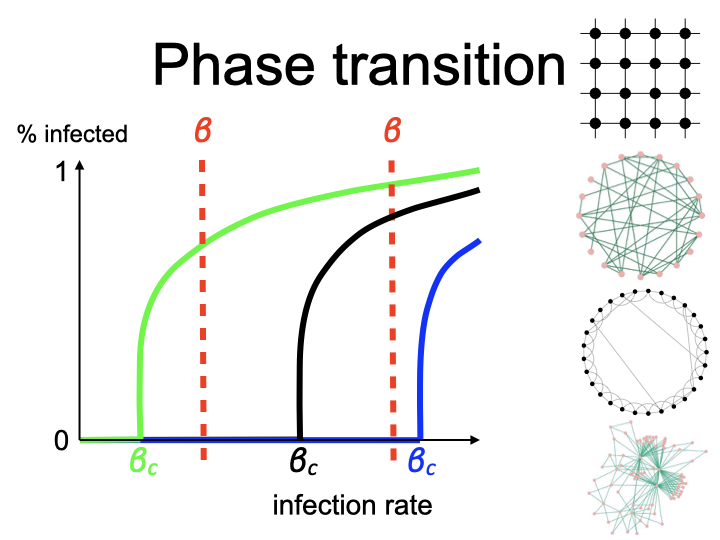
\includegraphics[width=0.75\textwidth]{figures/9_networks/phase-transition-from-slide.png}
\caption{Phase diagram of the SIS/SIR model.}
\end{center}
\end{figure}

\begin{itemize}
\item Epidemic threshold, $\beta_{\text{c}}$: large-scale spreading of infection occurs in the SIR model with a positive probability if $\beta > \beta_{\text{c}}$.
	\begin{itemize}
	\item Similar interpretation for the SIS model.
	\end{itemize}
\item A central result: under ``degree-heterogeneous mean-field approximation'' (where we assume that $N\to\infty$ and that nodes with the same degree $k$ behave in the same manner, which would hold true when the clustering coefficient, $C$, is tiny),
\[ \beta_{\text{c}} = \frac{\langle k\rangle}{\langle k^2 \rangle - \langle k \rangle} \mu, \]
where $\langle k \rangle$ is the mean degree and $\langle k^2 \rangle$ is the mean of $k^2$ over all nodes (i.e., second moment of the degree).
\end{itemize}

\noindent\textbf{Example 1:} If every node has the same degree, $k$ (called the random regular graph, including the well-mixed population for which $k=N-1$),
\[ \beta_{\text{c}} = \frac{\langle k\rangle}{\langle k^2 \rangle - \langle k \rangle} \mu = \frac{k}{k^2 - k} \mu = \frac{\mu}{k-1}. \]

\medskip
\noindent\textbf{Example 2:} For \emph{scale-free networks} (i.e., those with power-law $p(k)$), $\langle k^2 \rangle$ is much larger than $\langle k\rangle$ (and than $\langle k\rangle^2$). Then,
\[ \beta_{\text{c}} = \frac{\langle k\rangle}{\langle k^2 \rangle - \langle k \rangle} \mu \approx \frac{\langle k\rangle}{\langle k^2 \rangle} \mu \approx 0. \]
Then, an epidemic spreads even with a tiny infection rate $\beta$.
\begin{itemize}
\item Implications in HIV/AIDS transmission. Data:
\end{itemize}

\begin{figure}[h]
\begin{center}
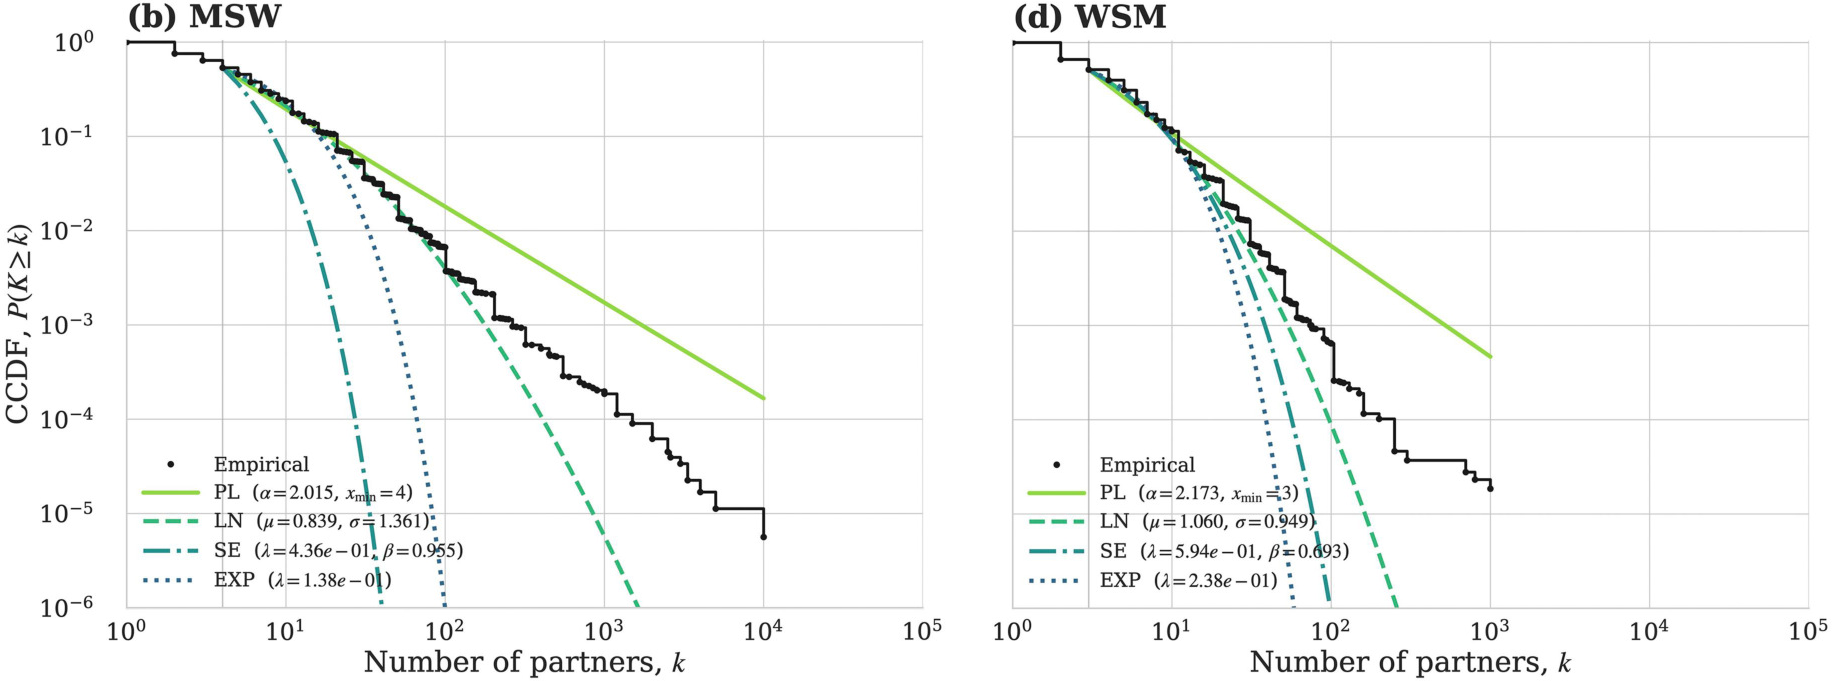
\includegraphics[width=\textwidth]{figures/9_networks/Arutkin2026-lifetime-partners.png}
\caption{Lifetime number of sex partners of UK Biobank participants aged 40--69, plotted as the fraction of participants with at least $k$ partners, $P(K\ge k)$ (CCDF: complementary cumulative distribution function). Left: men with female partners only. Right: women with male partners only. Figure~1(b) and (d) (cropped and placed side by side, with the vertical-axis labels taken from panel (a) and the horizontal-axis labels of panel (b) taken from panel (d)) of \hrefc{https://doi.org/10.3389/frph.2026.1790557}{Arutkin \& Vall\'ee, Frontiers in Reproductive Health, 8, 1790557 (2026)}, licensed under \hrefc{https://creativecommons.org/licenses/by/4.0/}{CC BY 4.0}. An earlier, classic data set of this kind is that of \hrefc{https://doi.org/10.1038/35082140}{Liljeros et al., Nature (2001)}.}
\end{center}
\end{figure}

\begin{itemize}
\item This surprising result comes from the friendship paradox.
	\begin{itemize}
	\item An infectious node tends to select a hub neighbor to transmit disease to. Once a hub gets infected, it would propagate the pathogen to many other nodes.
	\end{itemize}
\end{itemize}

\end{document}
